\documentclass{article}
\usepackage[utf8]{inputenc}
\usepackage{graphicx}
\usepackage{hyperref}
\usepackage{amsmath}
\usepackage{amssymb}
\usepackage{geometry}
\usepackage{float}
\geometry{a4paper, margin=1in}

\title{Computer Security Theory}
\author{Simone}
\date{}

\begin{document}

\maketitle

\section{Introduction}

Notebook

\section{Cryptography}

Tries to guarantee

\begin{figure}[H] \centering 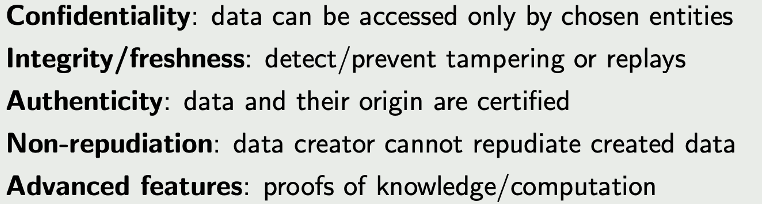
\includegraphics[width=0.8\textwidth]{media/image1.png} \end{figure}

The main problem addressed by cryptography is how to enable secure communication over an \textbf{untrusted channel}, such as the Internet.

\begin{figure}[H] \centering 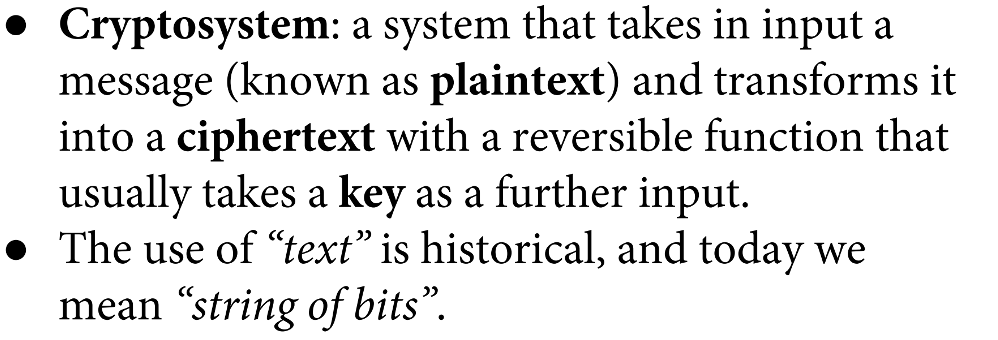
\includegraphics[width=0.8\textwidth]{media/image3.png} \end{figure}

\begin{figure}[H] \centering 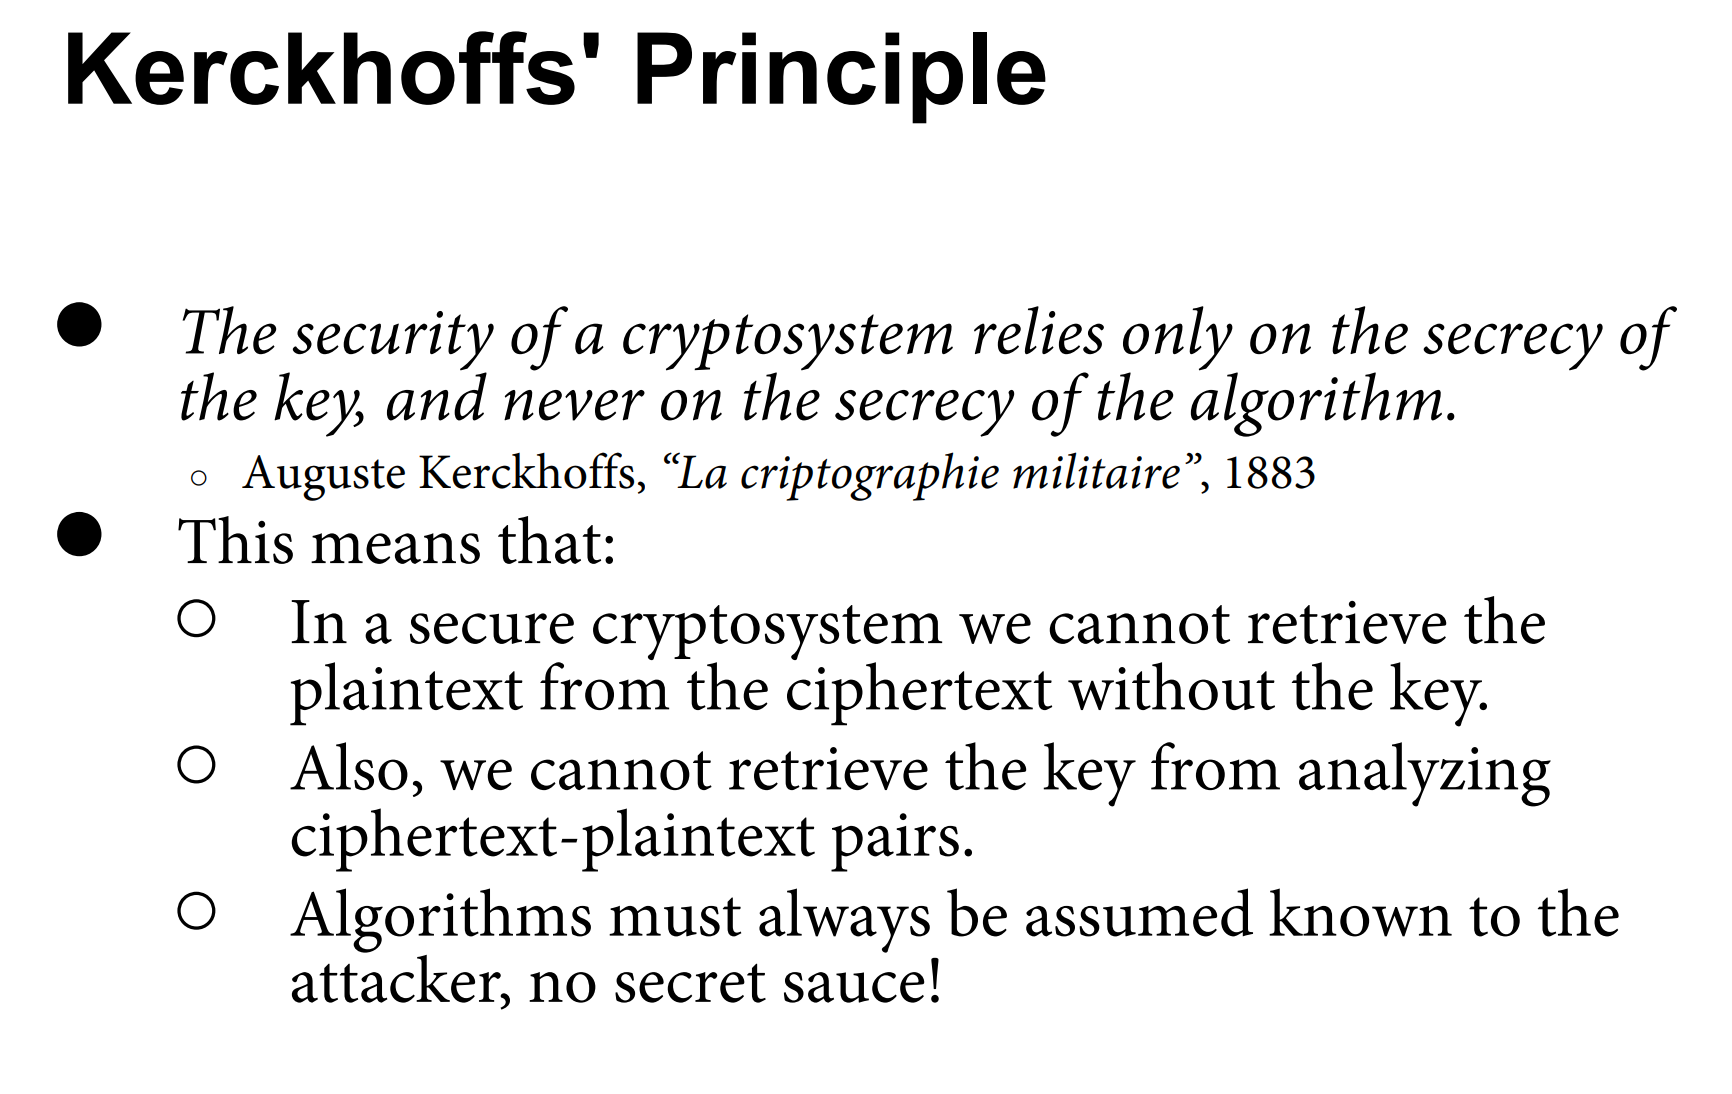
\includegraphics[width=0.8\textwidth]{media/image4.png} \end{figure}

Shannon showed that it is possible to construct a \textbf{mathematically unbreakable cipher}, however John Nash argued that in practice it is sufficient to use \textbf{computationally secure ciphers}

In cryptography, the \textbf{plaintext space (P)} is the set of all possible original messages that can be encrypted. In modern systems, these messages are typically represented as \textbf{bit strings}.

The \textbf{ciphertext space (C)} is the set of all possible encrypted messages produced after encryption.

A \textbf{cipher} is the cryptographic algorithm used to transform plaintext into ciphertext using a key. The resulting \textbf{ciphertext} is the encrypted form of the message, which appears unintelligible to anyone who does not possess the correct key.

The \textbf{key space (K)} is the set of all possible keys that can be used by the cipher, usually represented as bit strings of a certain length.

\begin{figure}[H] \centering 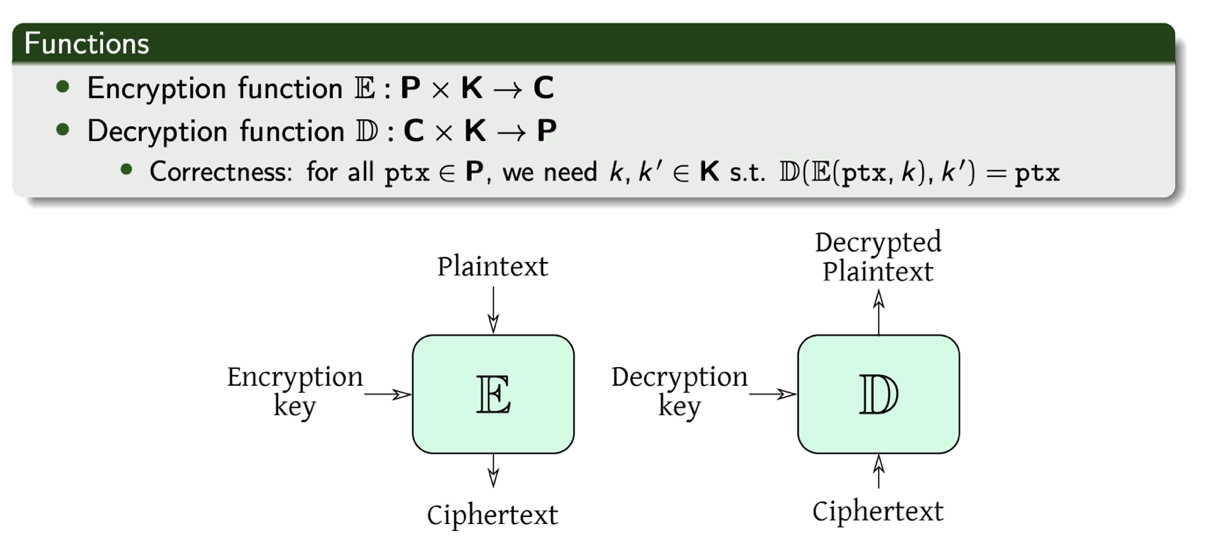
\includegraphics[width=0.8\textwidth]{media/image5.png} \end{figure}

The goal of cryptography in providing \textbf{confidentiality} is to ensure that only authorized parties can understand the transmitted data.

We can have three different attacker models:

\begin{enumerate}
    \item \textbf{Cyphertext-only attack}: the attacker can only sniff encrypted messages. The attacker is only an observer.
    \item \textbf{Known-plaintext attack}: the attacker knows some plaintext messages and their corresponding ciphertexts.
    \begin{enumerate}
        \item In a \textbf{chosen-plaintext attack} the attacker can choose specific plaintexts and obtain their corresponding encryptions. A cryptographic system is considered resistant to this type of attack if, even after observing the resulting ciphertexts, the attacker cannot distinguish which plaintext produced a given ciphertext.
    \end{enumerate}
    \item In \textbf{stronger models}, the attacker may tamper with data and observe the response of a decryption-capable entity, potentially even seeing the decrypted output.
\end{enumerate}

\subsection{Symmetric Encryption}

Technique used to ensure \textbf{confidentiality} of data.

In this model, the sender and the receiver share the \textbf{same secret key}, which is used both to encrypt and decrypt messages. Because both encryption and decryption rely on the same key, this approach is also called \textbf{shared-key encryption} or \textbf{secret-key encryption}.

A key requirement of symmetric encryption is that both parties must already possess the \textbf{same secret key} before secure communication can begin.

This introduces an important challenge known as the \textbf{key distribution problem}: the key must be exchanged through a \textbf{trusted channel} or another secure mechanism before it can be used. The key cannot be transmitted over the same untrusted channel used for encrypted communication, otherwise an attacker could intercept it.

Another issue is \textbf{scalability}, since each pair of users would need a unique shared key. This becomes infeasible when the number of users grows.

Every \textbf{Symmetric Encryption Algorithm combines two components}:

\begin{enumerate}
    \item Component based on \textbf{Substitution}: Replacing each byte with another one.
    \item Component based on \textbf{Transposition}: Positions of bits or characters are rearranged while their values remain unchanged.
\end{enumerate}

Check pages 22-23 for these components examples.

A \textbf{perfectly secure cipher} is a cryptographic system where observing the \textbf{ciphertext gives absolutely no information about the plaintext}.

Formally, this means that for every plaintext $ptx$ and ciphertext $ctx$, the probability that a given plaintext was sent \textbf{remains the same even after seeing the ciphertext}.

\begin{figure}[H] \centering 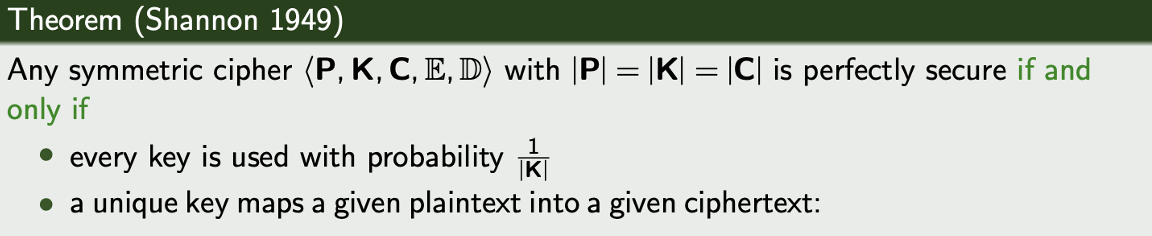
\includegraphics[width=0.8\textwidth]{media/image9.png} \end{figure}

\begin{figure}[H] \centering 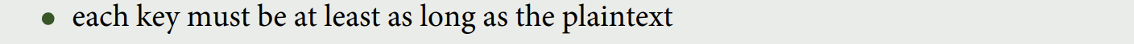
\includegraphics[width=0.8\textwidth]{media/image10.png} \end{figure}

\begin{figure}[H] \centering 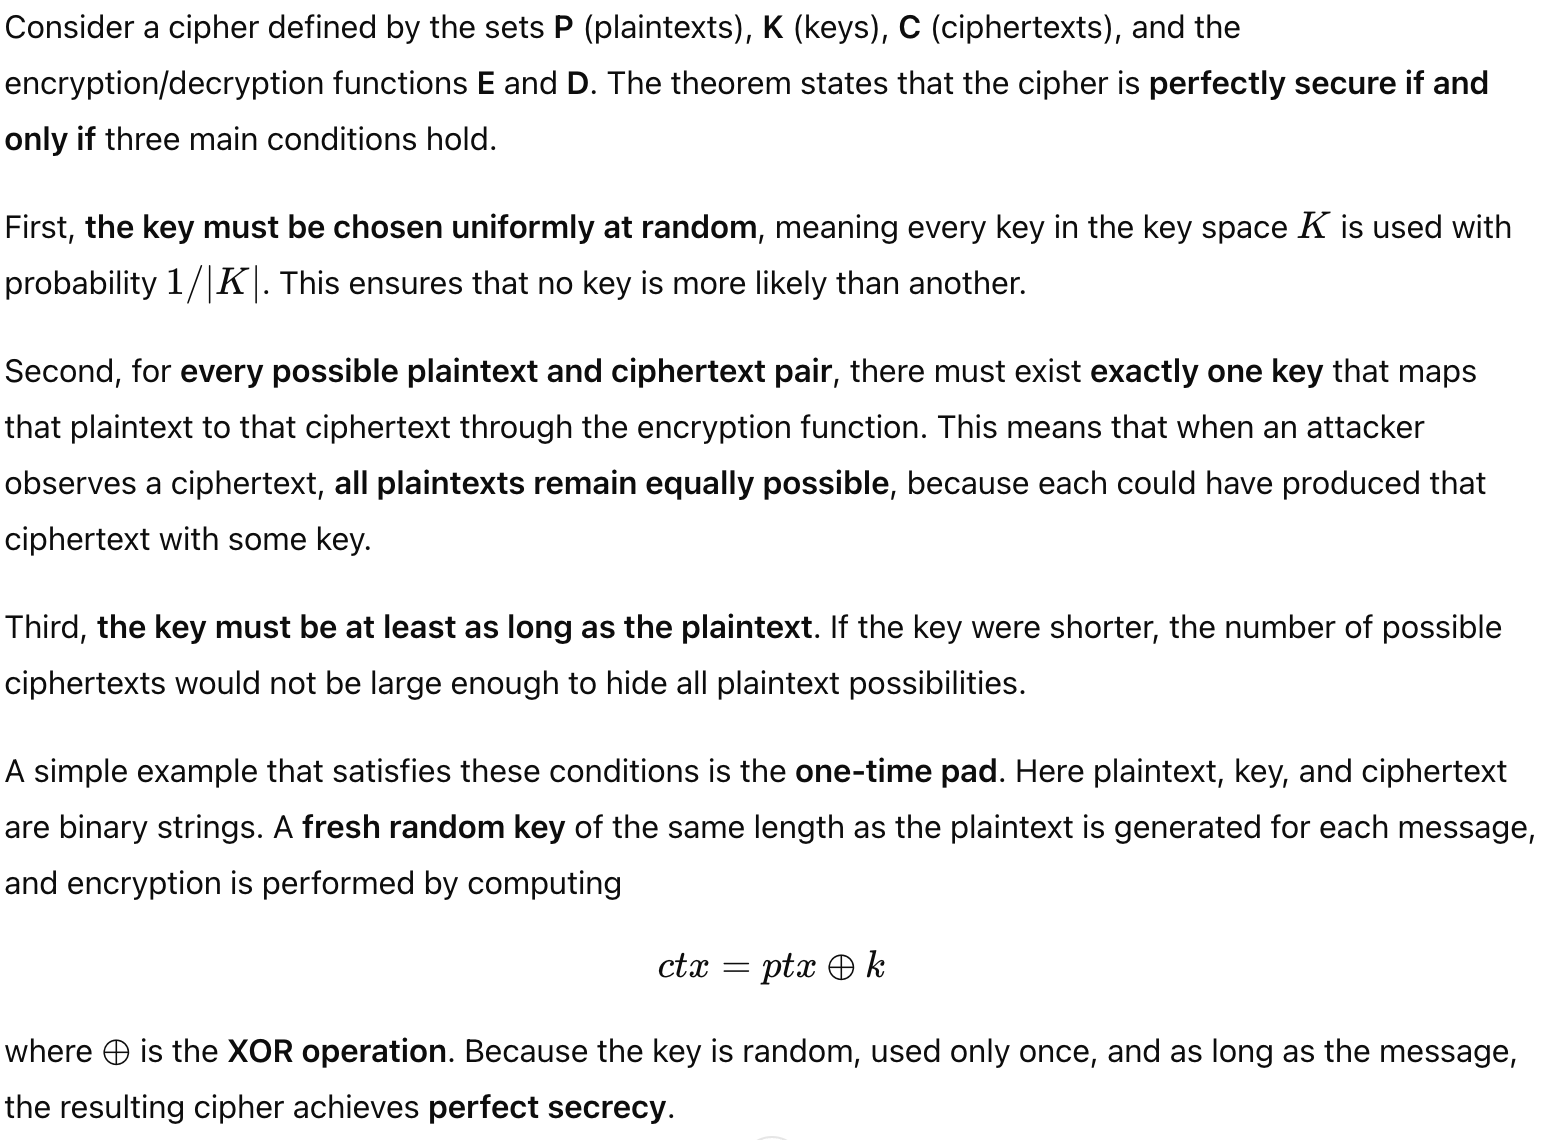
\includegraphics[width=0.8\textwidth]{media/image13.png} \end{figure}

The idea is:

\begin{enumerate}
    \item Take a \textbf{plaintext message} $p$.
    \item Use a \textbf{random key} $k$ of the \textbf{same length} as the message.
    \item Compute the ciphertext using \textbf{XOR}:
\end{enumerate}

$$c = p \oplus k$$

The key must be random, as long as the message and used only once. This system is a \textbf{perfect cipher}. The main problem is key management (huge size and huge number of keys). Furthermore, the system becomes insecure if key is stolen or reused. Additionally, generating truly random keys is challenging.

Hence, \textbf{Perfectly secure != Perfectly usable}

Because \textbf{Perfectly secure != Perfectly usable}, modern cryptography relies on \textbf{computationally secure ciphers} instead.

In real world scenarios, the cryptographic algorithms used are \textbf{not perfect}, mainly because the \textbf{key space is smaller than the plaintext space} ($| K | < | P |$).

Since keys are reused, each observed \textbf{plaintext--ciphertext pair leaks a small amount of information} about the key which, according to \textbf{Kerchoff's principle}, is the only secret part of the algorithm.

This is because \textbf{brute force attacks} are theoretically possible for any real world cipher. A real cryptosystem is \textbf{broken} if there is a way to break it \textbf{faster} than brute forcing.

Since perfect ciphers (impossible to break with brute force even with unlimited time and power) are unusable and not perfect ciphers can be broken by brute force attacks, the goal is to design a cipher such that breaking it would require solving a \textbf{very hard computational problem} efficiently.

Examples of such hard problems include:

\begin{itemize}
    \item \textbf{Solving nonlinear Boolean equation systems}
    \item \textbf{Factoring large integers}
    \begin{itemize}
        \item Computing $n = p \times q$ is easy, but is very slow finding $p$ and $q$ given $n$.
    \end{itemize}
    \item \textbf{Computing discrete logarithms}
    \begin{itemize}
        \item $x = \log_a(y) \Rightarrow$ it is difficult to compute $x$ knowing $y$.
    \end{itemize}
    \item \textbf{Decoding random linear codes or finding the shortest vector in a lattice} (used in some post-quantum cryptography)
\end{itemize}

To prove that a cryptographic scheme is secure, researchers typically follow three steps.

\begin{enumerate}
    \item \textbf{Define the ideal attacker behaviour.}\\
    We consider the strongest possible attacker, one who has unlimited computational resources and time.
    \item \textbf{Assume a computational problem is hard.}\\
    Security is based on the assumption that certain problems cannot be solved efficiently.
    \item \textbf{Reduction proof.}\\
    If we are not able to find any non-ideal attacker (an attacker with finite time) that solves the hard problem, it means that the algorithm is computationally secure.
\end{enumerate}

\subsubsection{Random and Pseudorandom Keys}

The \textbf{one-time pad} is perfectly secure, but it has a huge problem: the key must be:

\begin{itemize}
    \item truly random;
    \item as long as the message;
    \item used only once;
\end{itemize}

For this reason, in practice a short key, called a \textbf{seed}, is used and is "expanded" with a deterministic generator.

This generator is called \textbf{CSPRNG}, which stands for \textbf{Cryptographically Secure Pseudorandom Number Generator}.

A CSPRNG takes as input a short string:

\begin{figure}[H] \centering 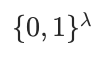
\includegraphics[width=0.8\textwidth]{media/image16.png} \end{figure}

and produces a longer string:

\begin{figure}[H] \centering 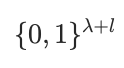
\includegraphics[width=0.8\textwidth]{media/image17.png} \end{figure}

where $l$ is the \textbf{stretch}, i.e., how much the key is lengthened.

The output is not truly random, because the generator is \textbf{deterministic}: if I use the same seed, I always get the same output. However, it must appear random to any efficient attacker.

So the fundamental idea is:

the output of the CSPRNG is not truly random, but it must be computationally indistinguishable from a truly random string.

"Computationally indistinguishable" means that an attacker working in \textbf{polynomial time} cannot tell whether they are seeing a truly random string or the output of the CSPRNG.

However, if the attacker had infinite time, they could distinguish the CSPRNG from a truly random source, because the CSPRNG has a finite number of possible seeds.

Finally, in practice we do not have an absolute mathematical proof of the existence of secure CSPRNGs. We use candidate constructions, considered secure based on computational assumptions. Often CSPRNGs are built using a building block:

\begin{itemize}
    \item PRP, pseudorandom permutations.
    \begin{itemize}
        \item In turn defined by \textbf{pseudorandom functions (PRFs)}.
    \end{itemize}
\end{itemize}

\paragraph{RF vs PRF vs PRP}

A \textbf{Random Function (RF)} is a function chosen randomly from all possible functions:

\begin{figure}[H] \centering 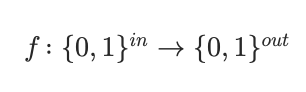
\includegraphics[width=0.8\textwidth]{media/image18.png} \end{figure}

This means it takes inputs of $in$ bits and produces outputs of $out$ bits.

The problem is that a truly random function would have to be stored as a huge table:

\begin{figure}[H] \centering 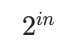
\includegraphics[width=0.8\textwidth]{media/image19.png} \end{figure}

rows, one for each possible input. Each row contains an output of $out$ bits. So it would require exponential memory. For example, with $in=128$, $2^{128}$ rows would be needed: impossible in practice.

For this reason, in cryptography we do not use truly random functions, but \textbf{Pseudorandom Functions (PRF)}.

A \textbf{PRF} is a deterministic function that depends on a secret key/seed:

\begin{figure}[H] \centering 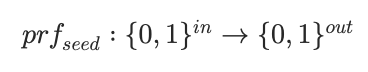
\includegraphics[width=0.8\textwidth]{media/image20.png} \end{figure}

Once the seed is fixed, the entire function is fixed. The advantage is that we do not have to save a huge table: it is enough to save a short key.

The important property is that an efficient attacker, that is, one working in polynomial time, cannot distinguish a PRF from a truly random function.

So:

PRF $\approx$ RF

from the point of view of an efficient attacker.

Then the \textbf{Pseudorandom Permutation (PRP)} is introduced, which solves the main problem of PRFs, namely that they are injective but not bijective.

A \textbf{PRP} is a special PRF that is also \textbf{bijective}, meaning:

\begin{figure}[H] \centering 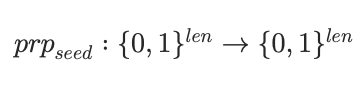
\includegraphics[width=0.8\textwidth]{media/image21.png} \end{figure}

Input and output have the same length, and each output corresponds to one and only one input.

This is fundamental because a PRP is \textbf{invertible}: I can go forward and also backward using the same key. This is why it is suitable for \textbf{block ciphers}, such as AES:

\begin{itemize}
    \item forward: encryption;
    \item backward: decryption.
\end{itemize}

Note one point: a generic PRF \textbf{does not necessarily have to be injective}. It can have collisions, especially if the output is smaller than or equal to the input. The bijective property is instead required for \textbf{PRPs}, not for all PRFs.

\textbf{Real} PRPs are built by applying simple but \textbf{bijective} boolean functions multiple times, combined with a \textbf{secret key}. The idea is to gradually increase complexity: after many rounds, the output must seem random and not linked to the input.

In practice, concrete PRPs are \textbf{block ciphers}. A block cipher takes a block of bits and returns another block of the same size. Being a permutation, it is invertible.

Security is evaluated through \textbf{public scrutiny}, i.e., public analysis. Modern algorithms are studied by many cryptographers, often after public competitions, and are subjected to cryptanalysis techniques to look for bias, weaknesses, or non-random patterns.

A PRP/block cipher is considered broken if an attacker, with fewer than:

$2^\lambda$

operations, manages for example to:

\begin{itemize}
    \item distinguish the cipher from a random permutation;
    \item recover the key;
    \item significantly reduce the number of plausible keys;
    \item find statistical irregularities in the output.
\end{itemize}

Here $\lambda$ is the length of the key in bits. If the key is $\lambda$ long, the key space is $2^\lambda$.

So a brute force would have to try up to $2^\lambda$ keys.

The final point is that the brute force time grows \textbf{exponentially} with $\lambda$.

\subsubsection{Block Ciphers}

A \textbf{block cipher} is a symmetric encryption algorithm that takes a \textbf{block of data of fixed length} and transforms it into another block of the \textbf{same length}, using a \textbf{secret key}.

The main block cipher today is \textbf{AES}. AES works on 128-bit blocks and can use 128, 192, 256-bit keys.

It was chosen by NIST after a public competition and is very efficient, partly because many modern processors have dedicated hardware instructions to accelerate it.

Before AES, \textbf{DES} was used, but today DES is considered insecure because it uses a key that is too short, 56 bits. So a brute force is realistically possible. To try to make it more secure, \textbf{Triple DES} was used, which applies DES multiple times, reaching about 112 bits of equivalent security. However, even Triple DES is now deprecated and remains only in old systems.

\paragraph{Operating Modes}

\textbf{Operating modes}, that is, how to use a block cipher on messages longer than a single block.

The simplest mode is \textbf{ECB}, Electronic Codebook. In ECB you divide the plaintext into blocks and encrypt each block separately with the same key.

The problem is that if two plaintext blocks are the same, then the two ciphertext blocks will also be the same. So ECB reveals the pattern and structure of the message. This is why it is not secure for long messages.

The best solution is \textbf{CTR mode}, Counter mode. In CTR you do not directly encrypt the plaintext blocks. Instead, you encrypt a sequence of counters with the block cipher:

$ks_0 = Enc_k(0)$\\
$ks_1 = Enc_k(1)$\\
$ks_2 = Enc_k(2)$

These outputs form a \textbf{pseudorandom keystream} and then you perform an XOR between the plaintext and the keystream.

So CTR transforms a block cipher, like AES, into something that resembles a stream cipher.

The advantage is that even if two plaintext blocks are the same, the ciphertexts will be different, because they are XORed with different keystreams:

\begin{figure}[H] \centering 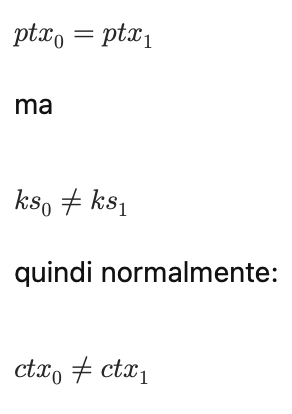
\includegraphics[width=0.8\textwidth]{media/image22.png} \end{figure}

The fundamental rule of CTR is:

you must never reuse the same counter with the same key.

If you reuse the same key-counter pair, you generate the same keystream. This is dangerous because it becomes similar to reusing the same key in the one-time pad, and it can leak information about the plaintexts.

\textbf{Example}

\begin{figure}[H] \centering 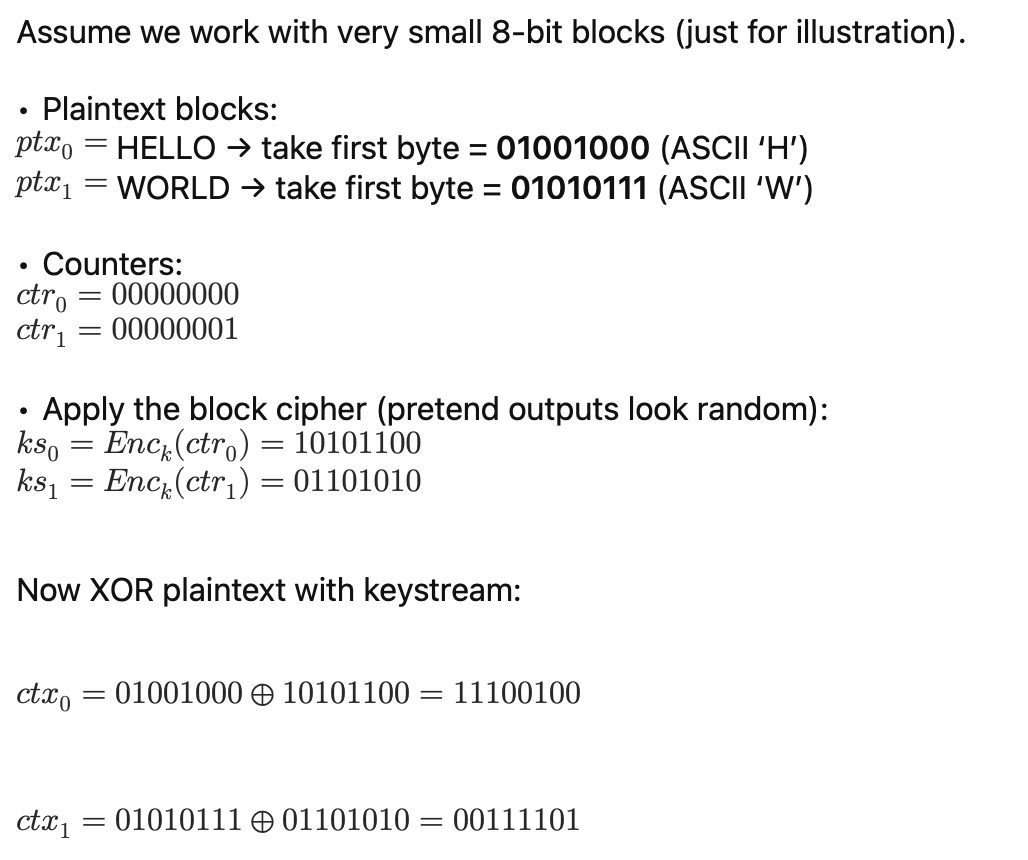
\includegraphics[width=0.8\textwidth]{media/image23.png} \end{figure}

In the case of a \textbf{ciphertext-only attack (CoA)}, the attacker only sees the ciphertexts. So they observe encrypted messages and try to derive information about the plaintext. In this scenario, modes like CTR can already provide good confidentiality, because the ciphertext seems random and does not show obvious patterns.

Then, however, a stronger attacker is considered: the \textbf{CPA} model, meaning \textbf{Chosen-Plaintext Attack}.

In a CPA attack, the attacker can choose some plaintexts and obtain their respective ciphertexts. In practice, they can query the encryption system as if they had access to an "encryption oracle".

The central point is that \textbf{deterministic} encryption is not enough for CPA security.

If the same plaintext always produces the same ciphertext, then the attacker can recognize when the same message is encrypted again. Thus, they can distinguish messages by comparing ciphertexts.

To achieve CPA security, the encryption must be \textbf{nondeterministic}, meaning it must introduce something that changes from one encryption to another.

There are three possible ways:

\begin{enumerate}
    \item % Empty item as in original
    \item \textbf{Rekeying}: changing/evolving the key for each block. It is possible, but often impractical.
    \item \textbf{Randomizing the encryption}: adding removable randomness in the encryption process, so the same plaintext can produce different ciphertexts.
    \item \textbf{Using a nonce}: in CTR mode, a \textbf{nonce} is used, meaning a number used once, as the starting point of the counter.
\end{enumerate}

In the case of CTR, instead of always starting from counter 0, a different nonce is chosen for each encryption. The nonce can be public, but it must be \textbf{unique} with that key.

The nonce can be public, but it must be unique.

\begin{figure}[H] \centering 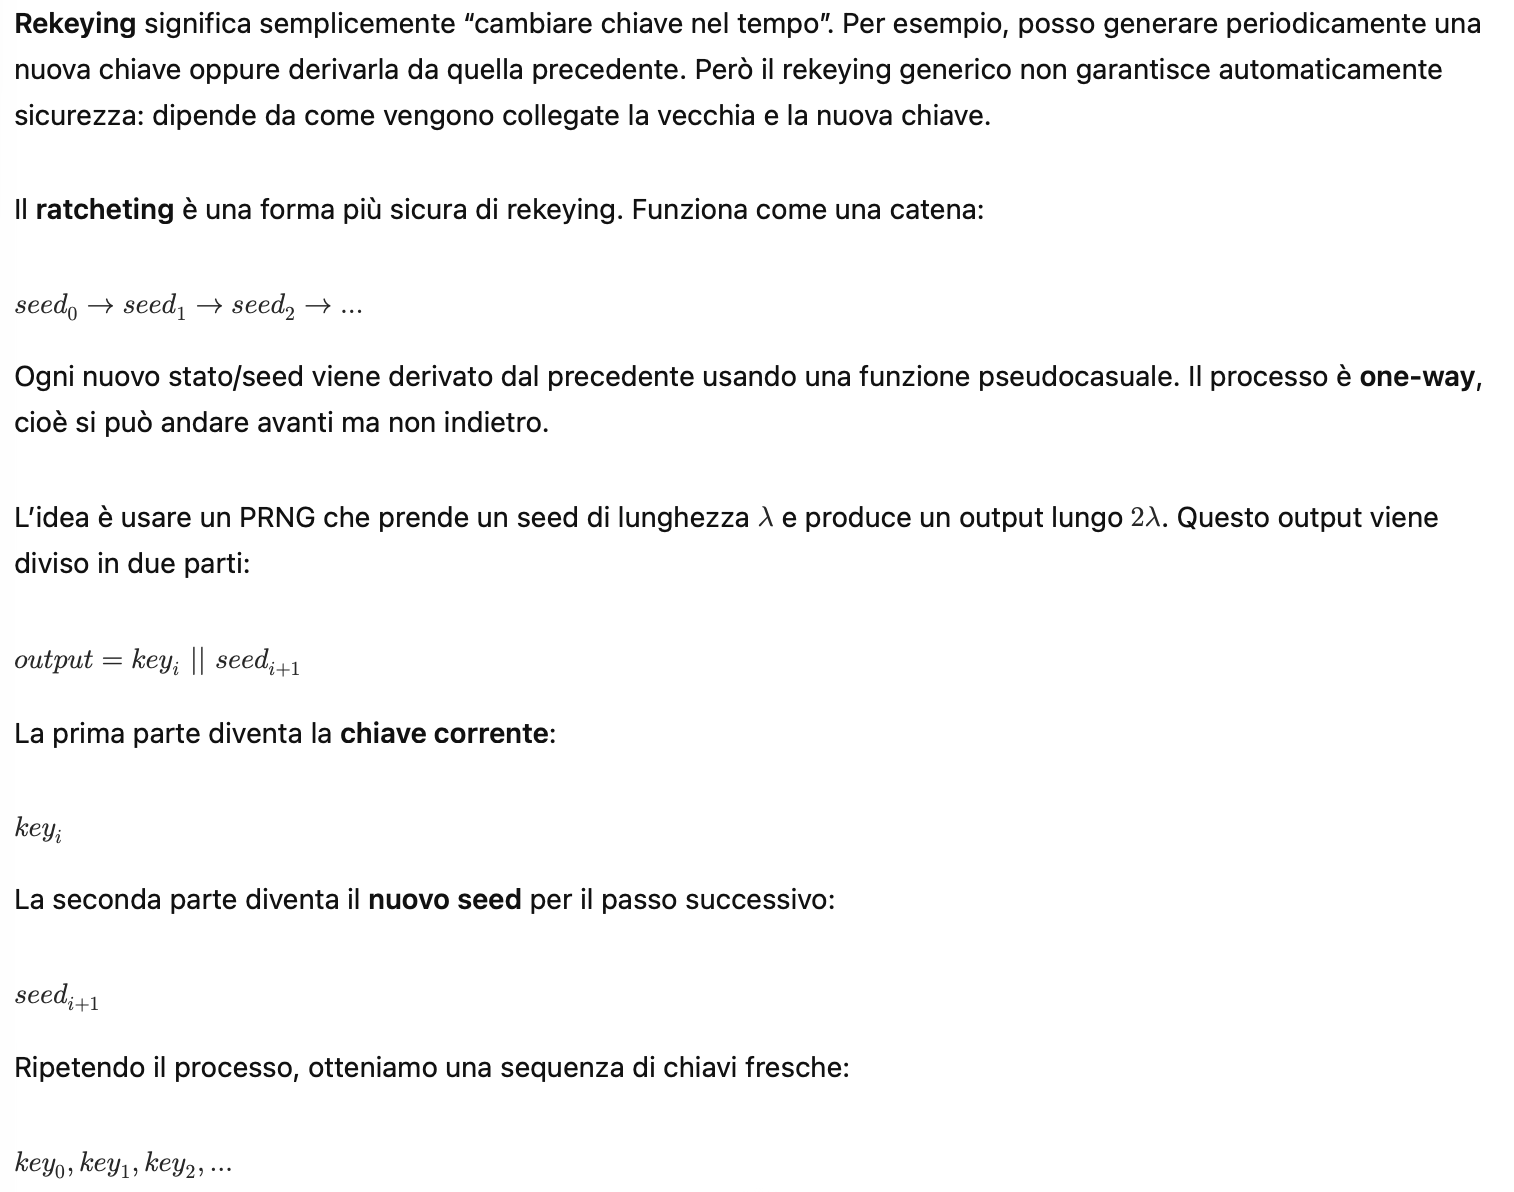
\includegraphics[width=0.8\textwidth]{media/image26.png} \end{figure}

\begin{figure}[H] \centering 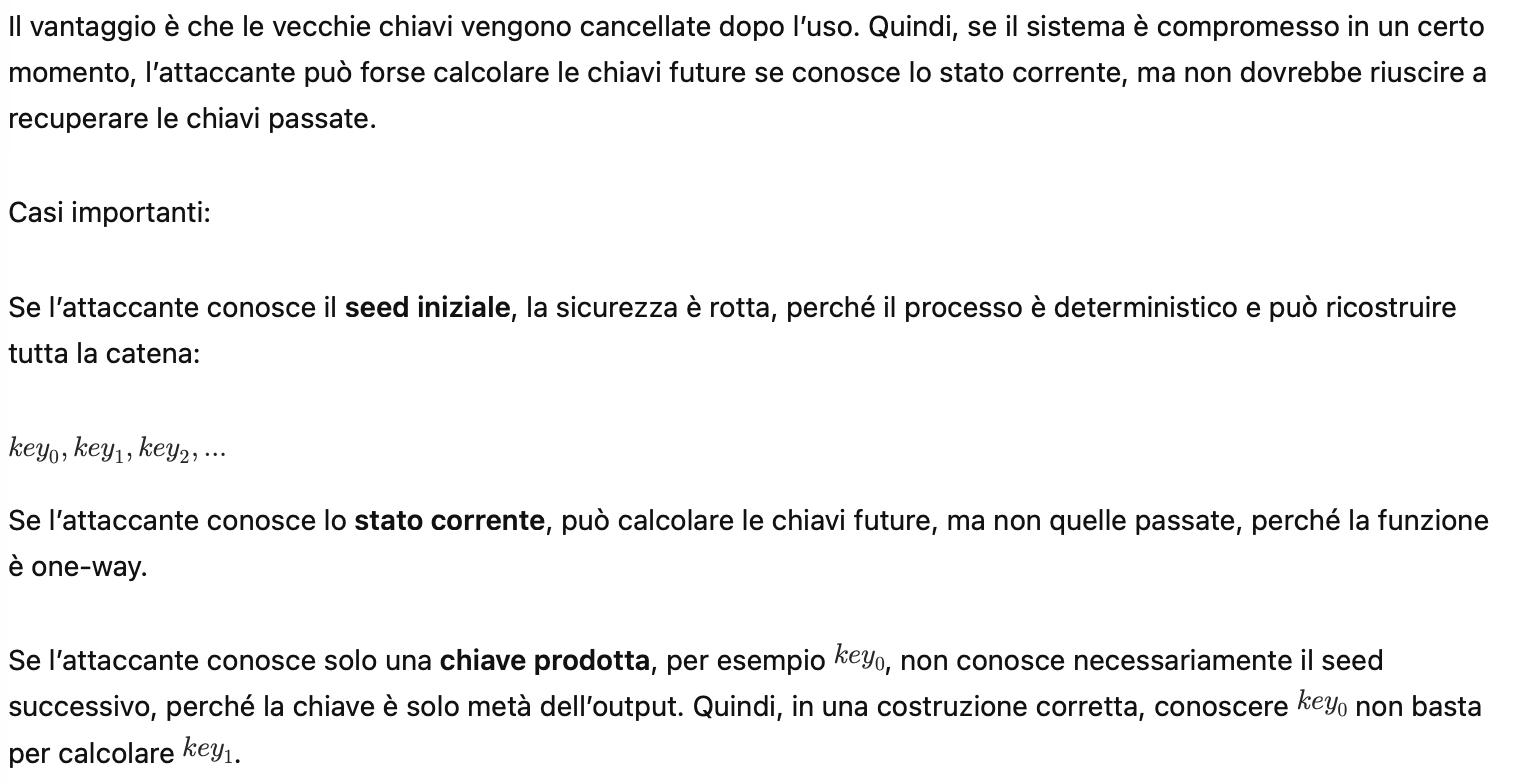
\includegraphics[width=0.8\textwidth]{media/image27.png} \end{figure}

\subparagraph{Malleability}

CTR protects \textbf{confidentiality}, meaning it prevents the attacker from reading the message.

However, it does not automatically protect \textbf{integrity}, meaning it does not prevent the attacker from modifying the message.

This problem is called \textbf{malleability}.

In a malleable encryption, the attacker does not know the plaintext, but they can modify the ciphertext in order to cause predictable changes in the plaintext after decryption.

In the case of CTR:

$ctx = ptx \oplus keystream$

If the attacker modifies a bit of the ciphertext, after decryption the corresponding bit of the plaintext changes. Thus, they can alter the message without knowing the key.

Conceptual example:

Pay 10 becomes Pay 90 if the attacker manages to modify the right bits.

Therefore:

encryption $\neq$ integrity
Encryption alone hides the content, but does not guarantee that the message has not been modified.

\paragraph*{MACs}

To guarantee integrity, a \textbf{MAC} is used, which is \textbf{Message Authentication Code}.

A MAC produces a small value called \textbf{tag}, calculated on the message using a secret key.

A \textbf{MAC has two main functions}:
\begin{itemize}
\item \textbf{generates the tag} t of the message m.
\item \textbf{checks if the tag is valid}.
\end{itemize}

The receiver verifies the tag: if the message has been modified, the verification should fail.

The attacker can also see many examples of pairs (m,t), meaning messages with their respective valid tags but, despite this, \textbf{must not be able to perform a forgery}, meaning to produce a new valid tag for a new message never seen before.

Even combining pieces of messages and previously seen tags to create a new valid pair is considered an attack.

\textbf{Important Note}

The MAC requires that the sender and receiver \textbf{know the same secret key}.

\begin{figure}[H] \centering 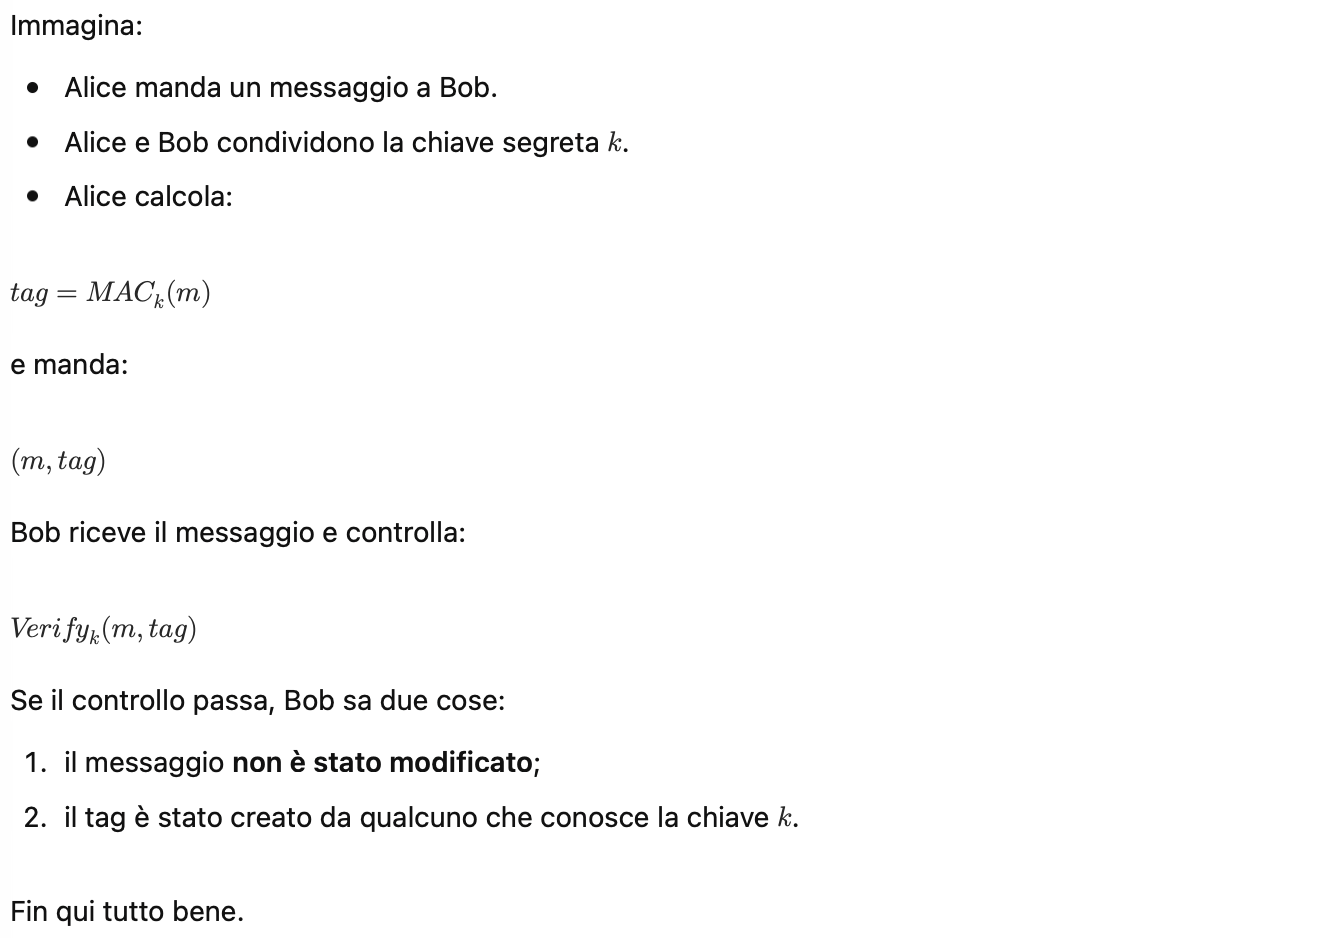
\includegraphics[width=0.8\textwidth]{media/image28.png} \end{figure}

However, this also means that whoever verifies the tag could, in theory, generate valid tags. Therefore, MACs guarantee \textbf{integrity and symmetric authenticity}, but do not guarantee \textbf{non-repudiation}.

\begin{figure}[H] \centering 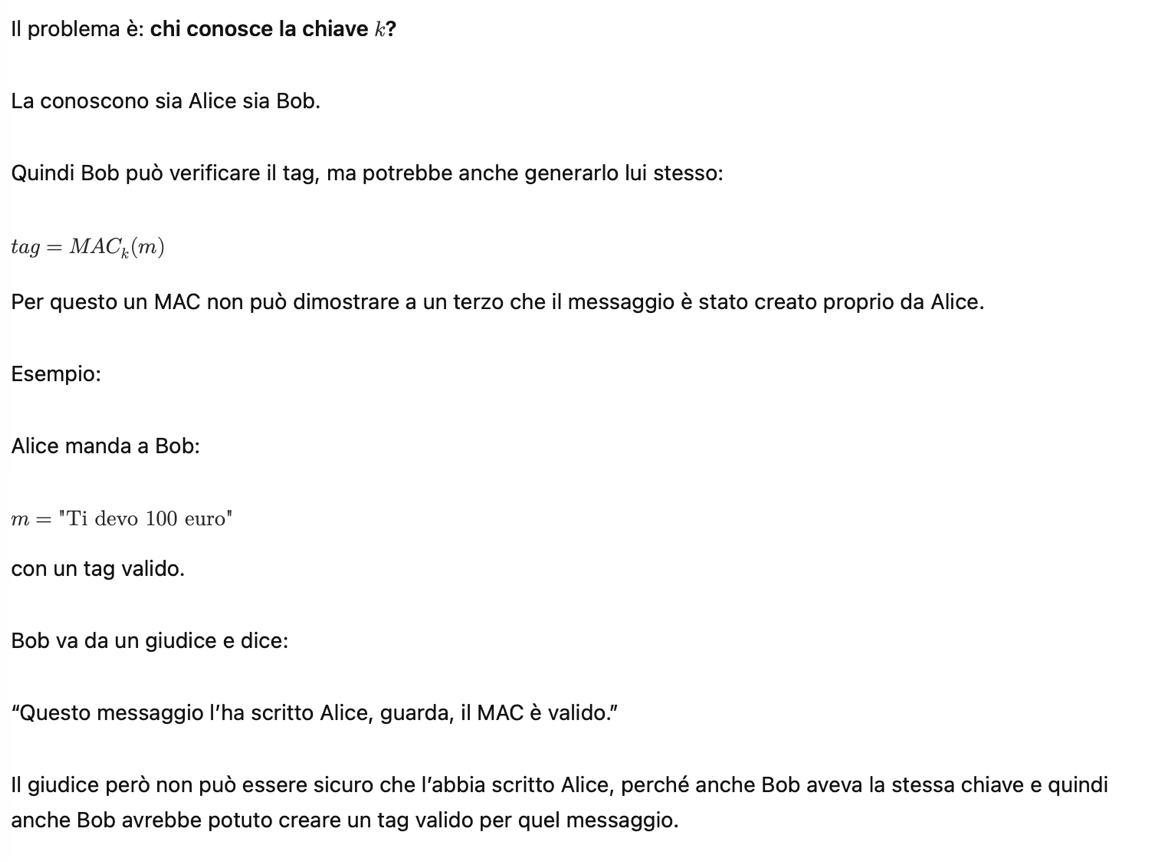
\includegraphics[width=0.8\textwidth]{media/image29.png} \end{figure}
Meaning: you cannot prove to a third party that only the sender created that message, because the receiver also had the key to generate the tag.

A common way to build a MAC is the \textbf{CBC-MAC (Cipher Block Chaining MAC)}. The idea is to process the message block by block, chaining the computations together.

\begin{figure}[H] \centering 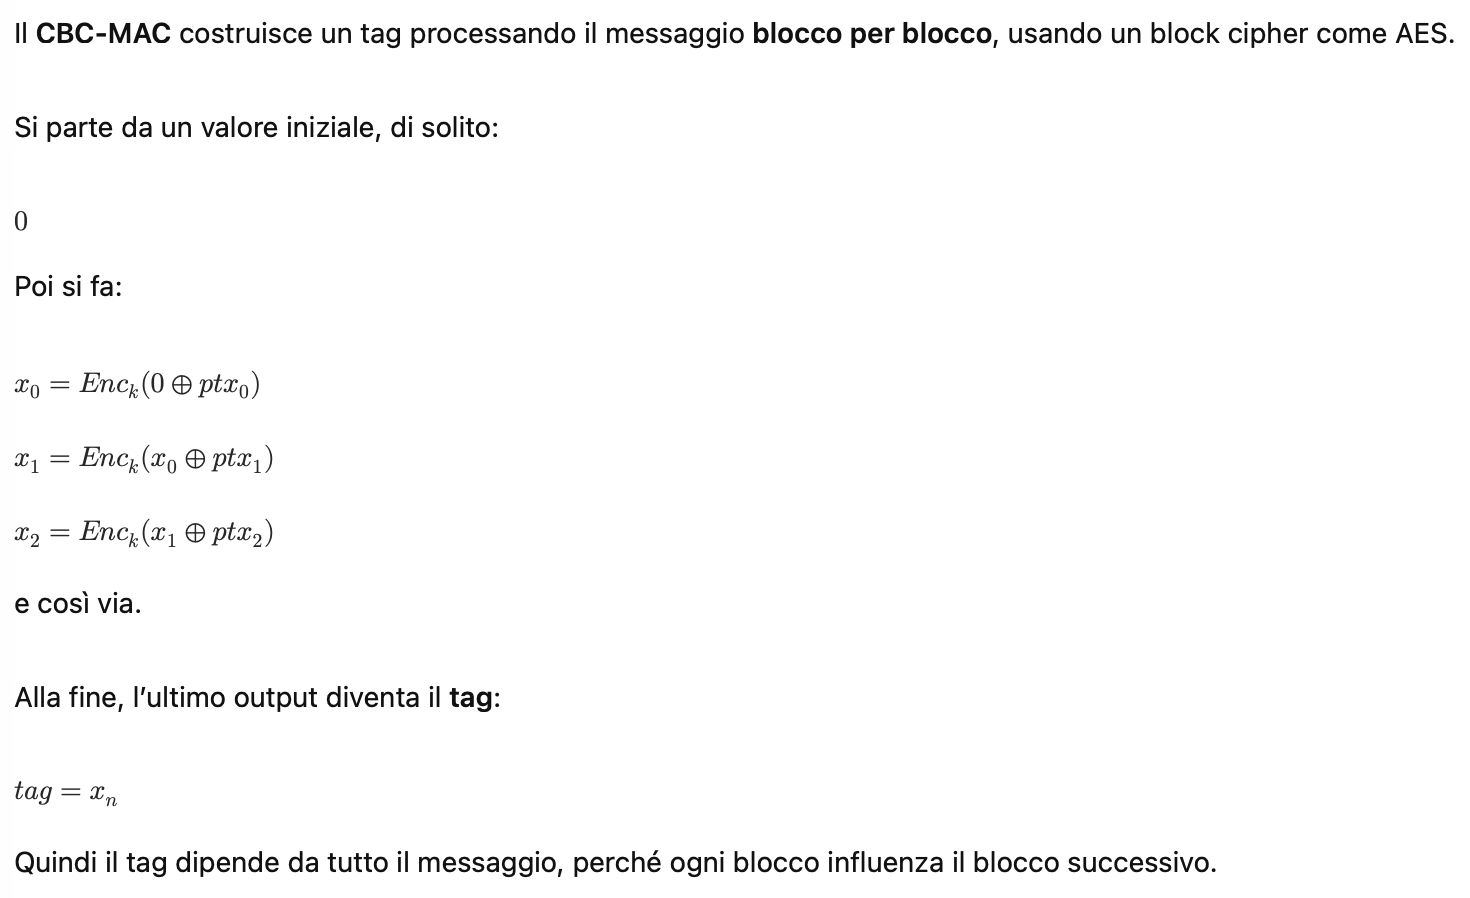
\includegraphics[width=0.8\textwidth]{media/image30.png} \end{figure}

The simple CBC-MAC is secure only under certain conditions, for example if the messages are \textbf{prefix-free} or have a \textbf{fixed length}.

\textbf{Prefix-free} means that a valid message cannot be a prefix of another valid message.

Non prefix-free example:

$m = \text{"pay 10"}$

$m' = \text{"pay 10 tomorrow"}$

Here $m$ is the beginning of $m'$.

The problem arises because in CBC-MAC the final tag is also the \textbf{final state} of the computation.

Therefore, if an attacker knows a valid pair they can use t as if it were \textbf{the new initial value} and continue the computation on other blocks.

A B C TAG1, if I have A B C D TAG2, to obtain TAG2 I just need to resume the computation from TAG1.

In this way, they can construct a valid tag for a longer message without knowing the key. This is called an \textbf{extension attack}.

\textbf{Why "prefix-free" helps}

If the system only accepts \textbf{prefix-free} messages, the attacker cannot take a valid message and transform it into a longer valid message.

So the extension attack does not work, because the extended message would not be accepted by the system.

\textbf{Why encrypting the tag again helps}

A possible fix is to encrypt the final result once more:

This way the attacker no longer directly sees the \textbf{final internal state} of the CBC-MAC.

They only see a transformed/encrypted version of the state. Therefore, they cannot reuse the tag as a starting point to continue the chain.

In practice, this breaks the extension attack.

MACs can be used, for example, as cookies or as SYN cookies.

\paragraph*{Hash Functions}

MACs guarantee integrity, but to verify a large file you still have to process the entire file.

For example, if I receive a 10 GB file and I want to verify the MAC, I have to recalculate the MAC on all 10 GB.

So the cost grows with the size of the message.

The ideal would be to have a \textbf{short} and \textbf{fixed value} that \textbf{represents the entire file}, \textbf{regardless} of its \textbf{size}.

This idea leads to \textbf{hash functions}.

A \textbf{hash function} is a function:

$H(x)=h$

that takes an input of arbitrary length and produces an output of fixed length.

The output is called \textbf{hash}, \textbf{digest} or \textbf{fingerprint}.

The digest is much shorter than the original message, but it should represent it reliably.

\textbf{Why they are needed}

Instead of comparing two files bit by bit, I can compare their hashes.

If I have a reliable digest $h$ received through a secure channel, and then I receive the file through an insecure channel, I can obtain the hash of the received file and compare it with $h$.

If they match, I assume the file has not been modified. If they are different, the file has been altered.

This is efficient because the digest has a constant size, independent of the file size.

\textbf{The problem is that collisions are inevitable}

Since the input can have arbitrary length, but the output has fixed length, collisions necessarily exist.

A \textbf{collision} occurs when two different inputs produce the same digest. So the goal is not to eliminate collisions, because it's impossible. The goal is to make them \textbf{computationally difficult to find}.

\textbf{The three security properties of cryptographic hashes}

A secure cryptographic hash must make three types of attack difficult.

\textbf{1. Preimage resistance}

Given the hash, I must not be able to trace back to a message that produces it.

It's a kind of "non-invertibility".

\textbf{2. Second preimage resistance}

If I know a message, I must not be able to find a different one with the same hash.

This protects against the attack where someone takes a valid document and looks for an alternative document with the same digest.

\textbf{3. Collision resistance}

It must be difficult to find any pair of different inputs that give the same hash.

Here the attacker does not start from a specific message: they can freely choose both inputs.

Second preimage = given a message, find me another one with the same hash

Collision = find any two messages with the same hash

\begin{figure}[H] \centering 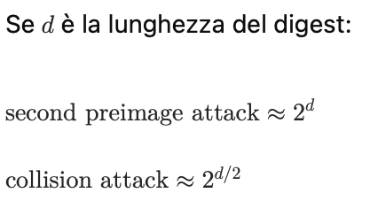
\includegraphics[width=0.8\textwidth]{media/image31.png} \end{figure}
This property is weaker in terms of attack cost, because thanks to the \textbf{birthday paradox} finding a collision requires about:

$2^{d/2}$ attempts, not $2^d$.

\textbf{When a hash is considered broken}

A hash function can be considered broken if an attacker is able to find:
\begin{itemize}
\item a preimage faster than brute force;
\item a second preimage faster than brute force;
\item a collision faster than the expected birthday attack.
\end{itemize}

So the problem is not just "finding a collision", because collisions always exist. The problem is finding them \textbf{too fast} compared to the expected security.

\begin{figure}[H] \centering 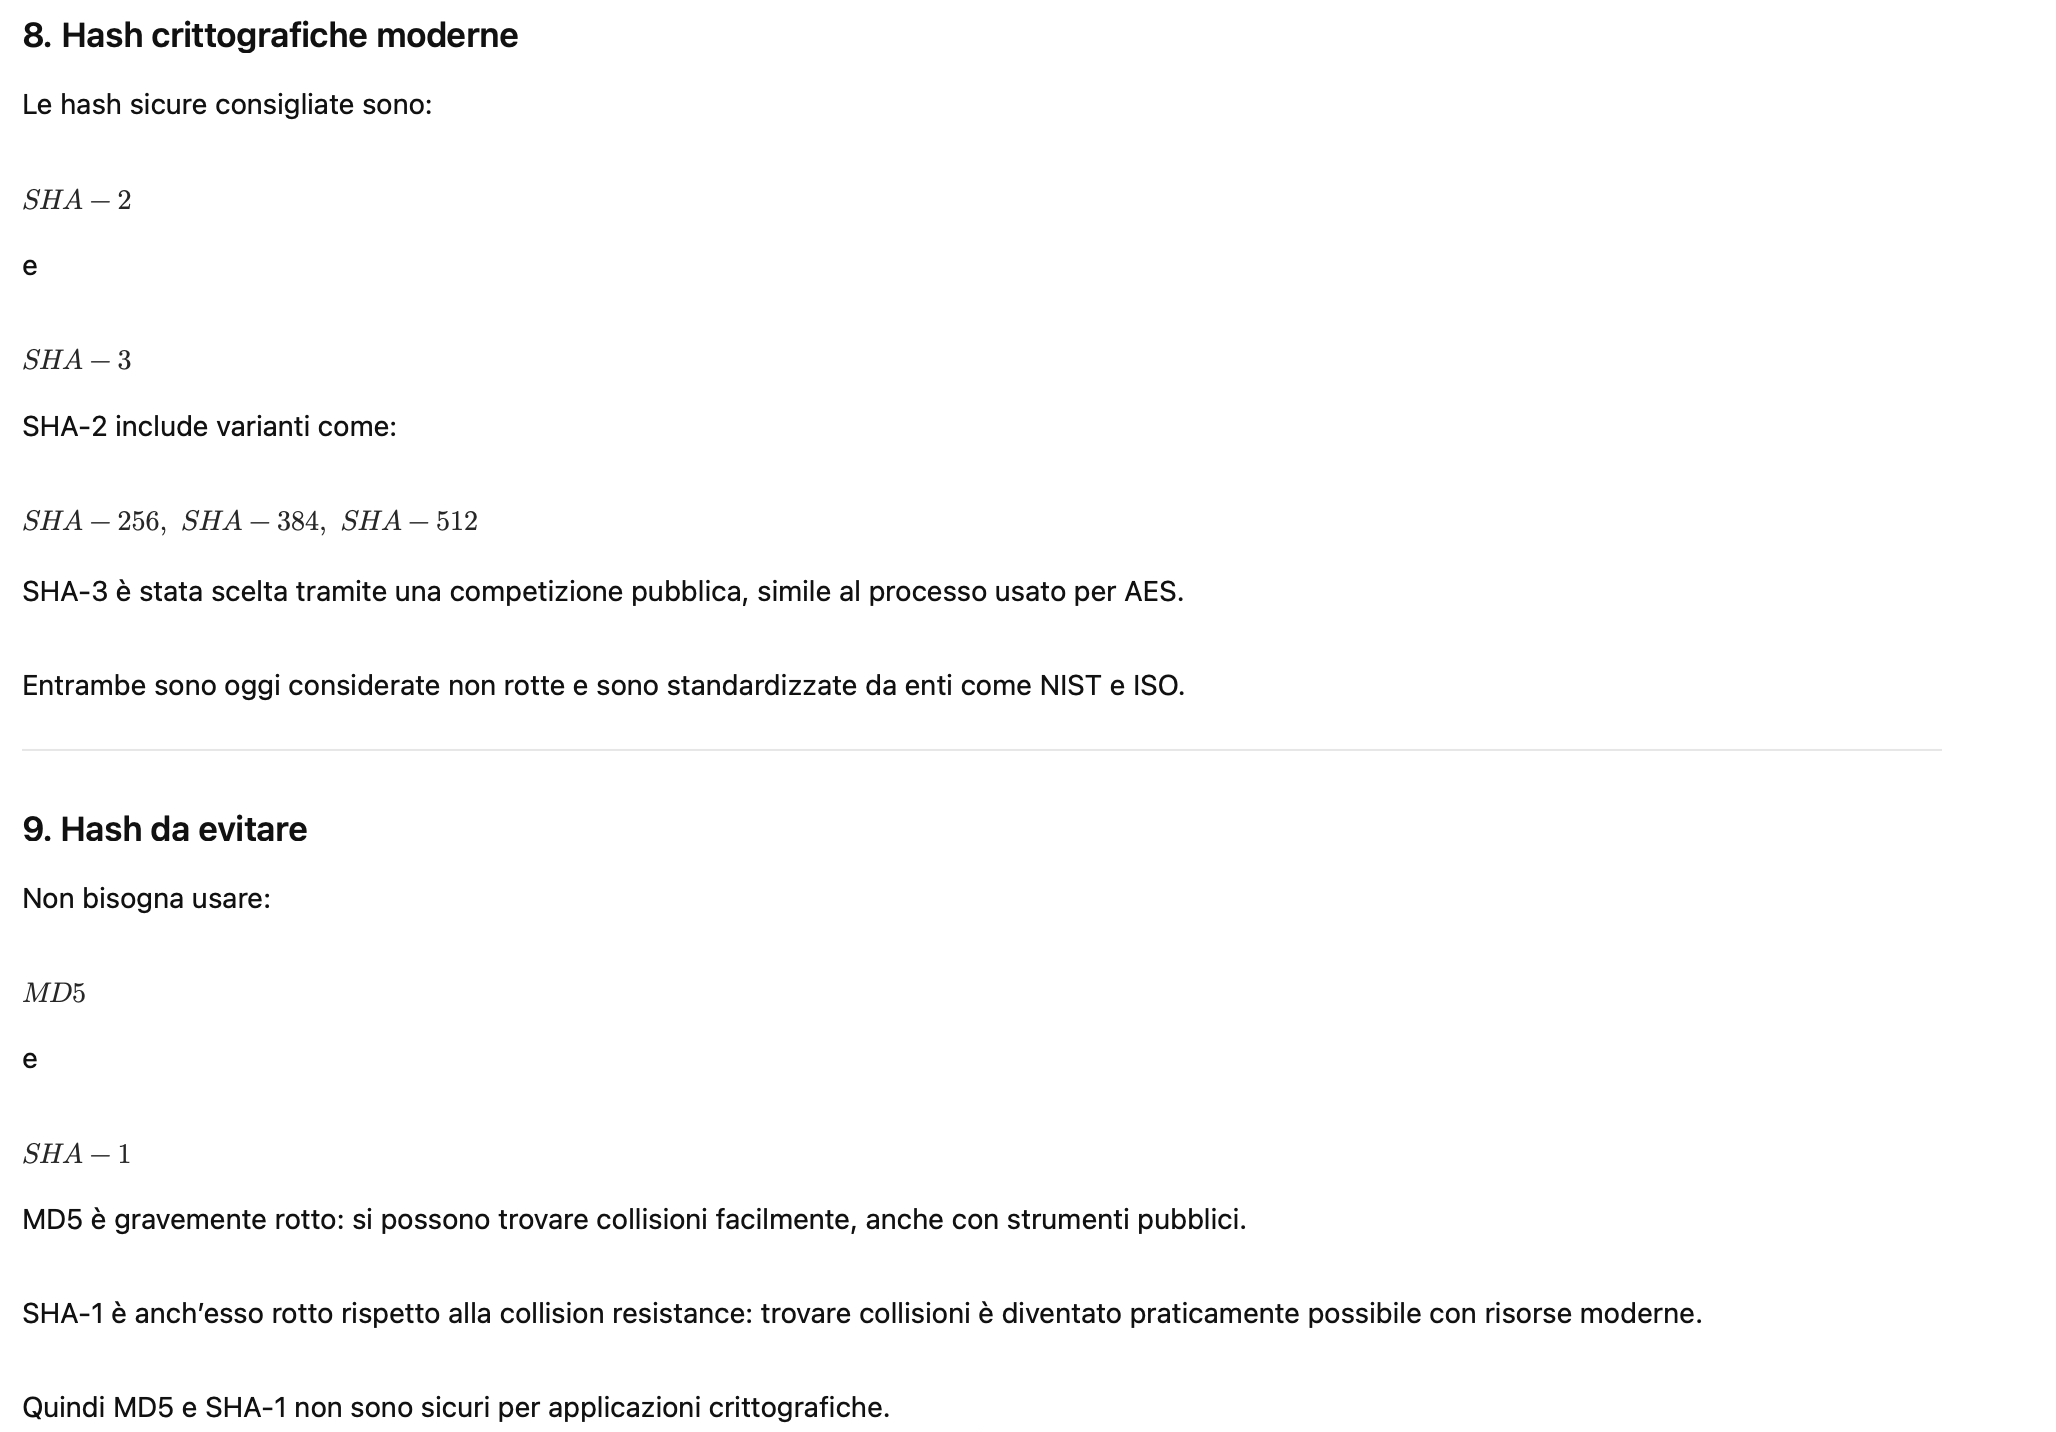
\includegraphics[width=0.8\textwidth]{media/image32.png} \end{figure}

\textbf{Practical uses of hash functions}

Hash functions are used in various contexts.

\textbf{Pseudonymized matching}

Instead of directly comparing sensitive data, their hashes are compared.

Example: if two users want to figure out if they have a common contact, they can compare hashes of phone numbers instead of the numbers in plaintext.

However, be careful: this improves privacy, but it is not always sufficient if the inputs are predictable, such as phone numbers or emails.

\textbf{MAC Construction: HMAC}

Hashes can be used to construct MACs.

The standard and secure construction is called \textbf{HMAC}.

The idea is to combine:

Message + Secret Key

in a controlled manner and calculate a tag.

HMAC is standardized and used with hashes like SHA-2 and SHA-3.

An important note from the slides: even though SHA-1 is not recommended as a generic hash, \textbf{HMAC-SHA1} can still be considered acceptable in some contexts, because the security of HMAC does not exactly coincide with the pure collision resistance of the hash.

\textbf{Forensic use}

In forensics, the hash is used to prove that a file or a disk image has not been modified.

For example, when acquiring a copy of a disk, its hash is noted in the official documents. Later, by recalculating the hash, it can be verified that the data remained identical.

\subsection*{Asymmetric Encryption}

The problem:

how do two people establish a secret key if they can only communicate over a public channel?

The breakthrough comes with \textbf{asymmetric cryptography}, which allows to:
\begin{itemize}
\item agree on a secret over a public channel;
\item send confidential messages without already having a shared key;
\item obtain strong authentication through digital signatures.
\end{itemize}

The main ideas are:

Diffie-Hellman key agreement

Public-key encryption

Digital signatures

\subsubsection*{Diffie-Hellman}

Diffie-Hellman is a \textbf{key agreement} protocol, meaning a protocol that allows two parties to obtain the \textbf{same shared secret key} communicating only over a public channel.

\begin{figure}[H] \centering 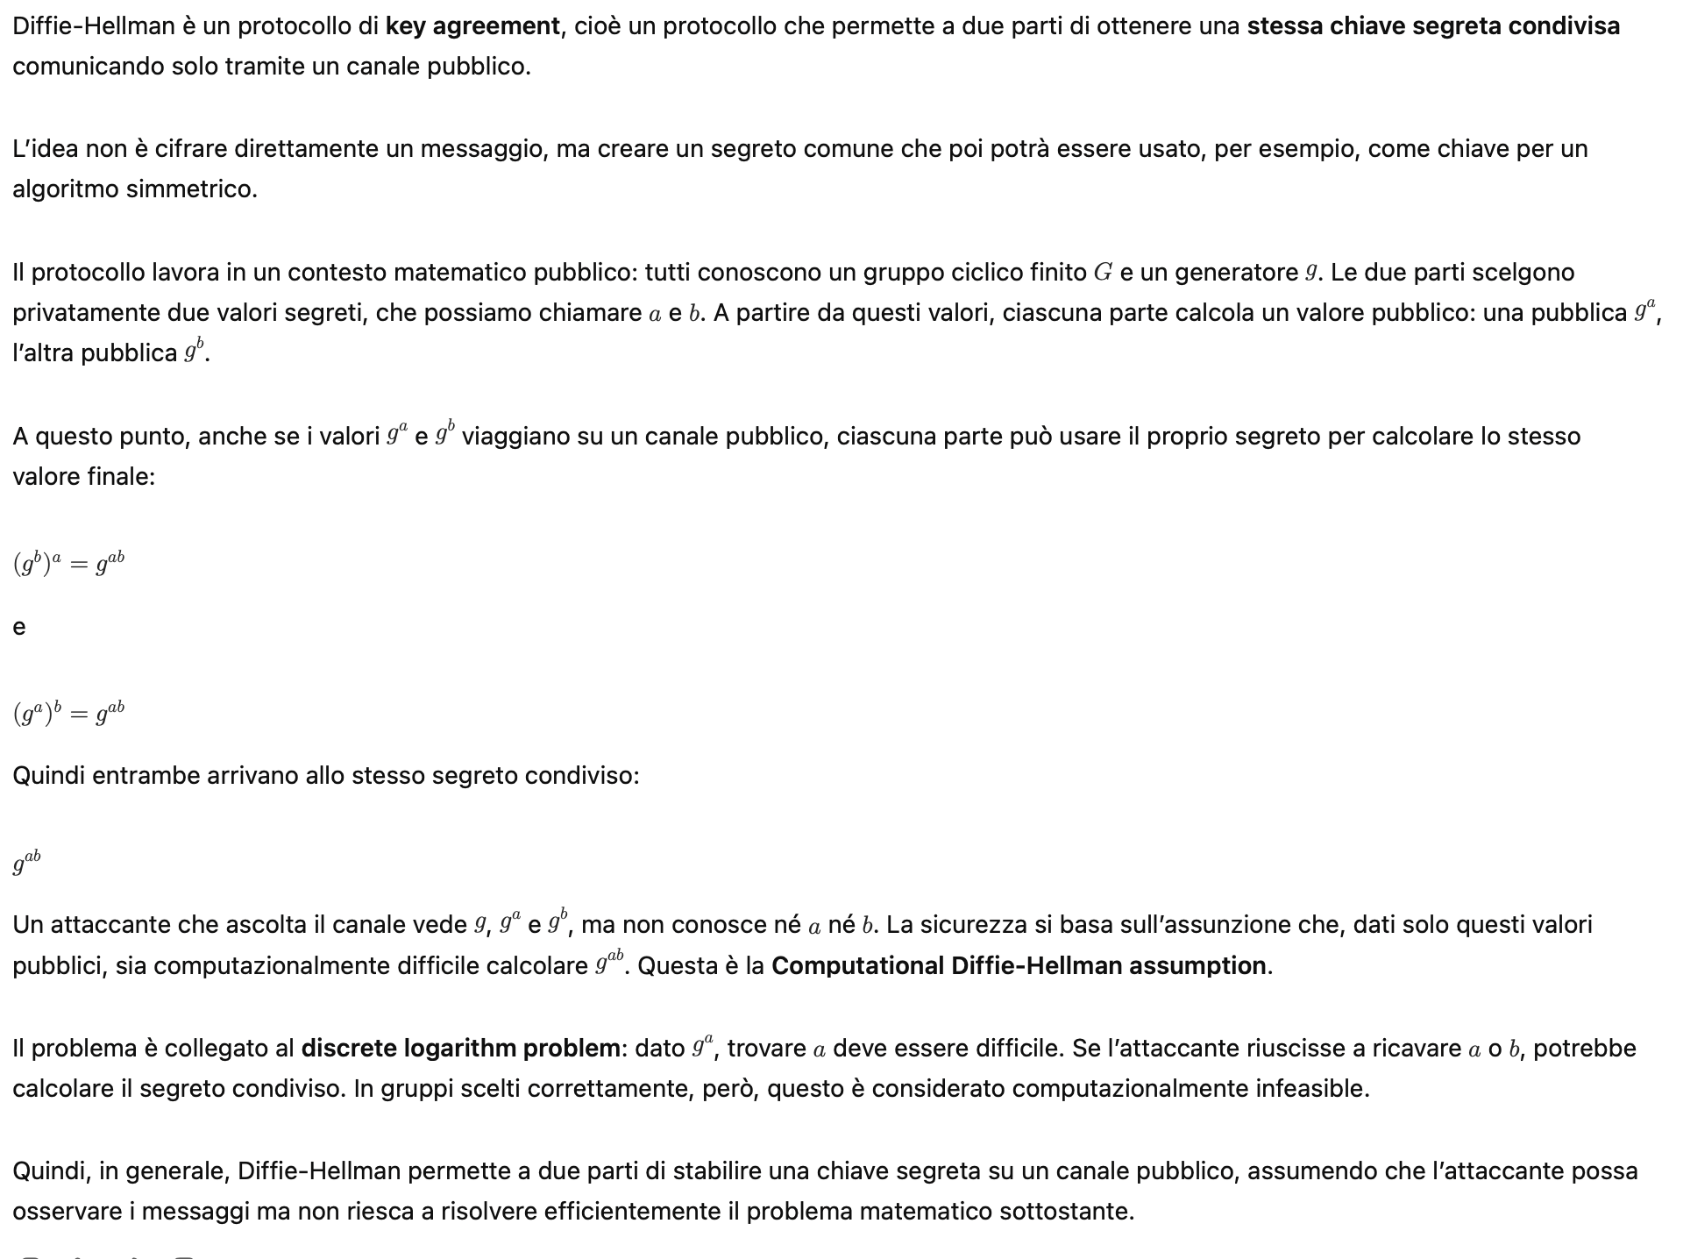
\includegraphics[width=0.8\textwidth]{media/image33.png} \end{figure}
The idea is not to directly encrypt a message, but to create a common secret that can then be used, for example, as a key for a symmetric algorithm.

\subsubsection*{Public Key}

\begin{figure}[H] \centering 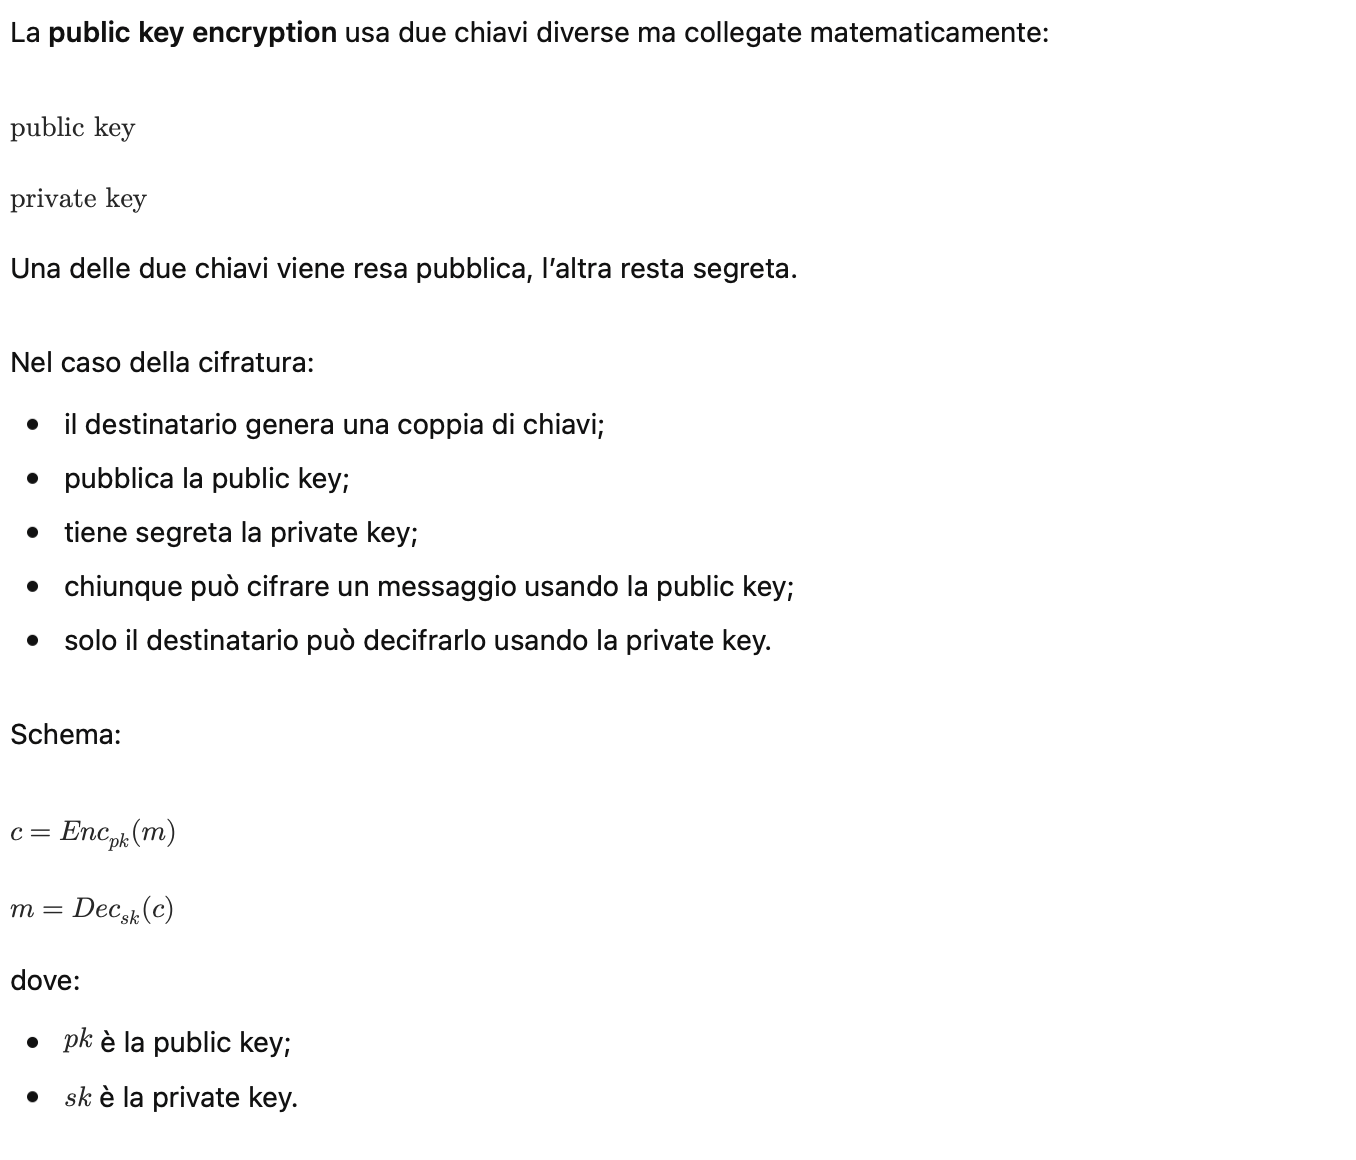
\includegraphics[width=0.8\textwidth]{media/image34.png} \end{figure}

But pay attention:

Public key encryption guarantees confidentiality, but alone it does not guarantee authenticity.

Anyone can use your public key to send you an encrypted message. So you know that only you can read it, but you don't automatically know who sent it.

To authenticate the sender, additional mechanisms are needed, such as \textbf{digital signatures}.

\subsubsection*{Key Length}

In both symmetric and asymmetric algorithms, the key length is measured in bits, but these bits do not mean the same thing.

\begin{figure}[H] \centering 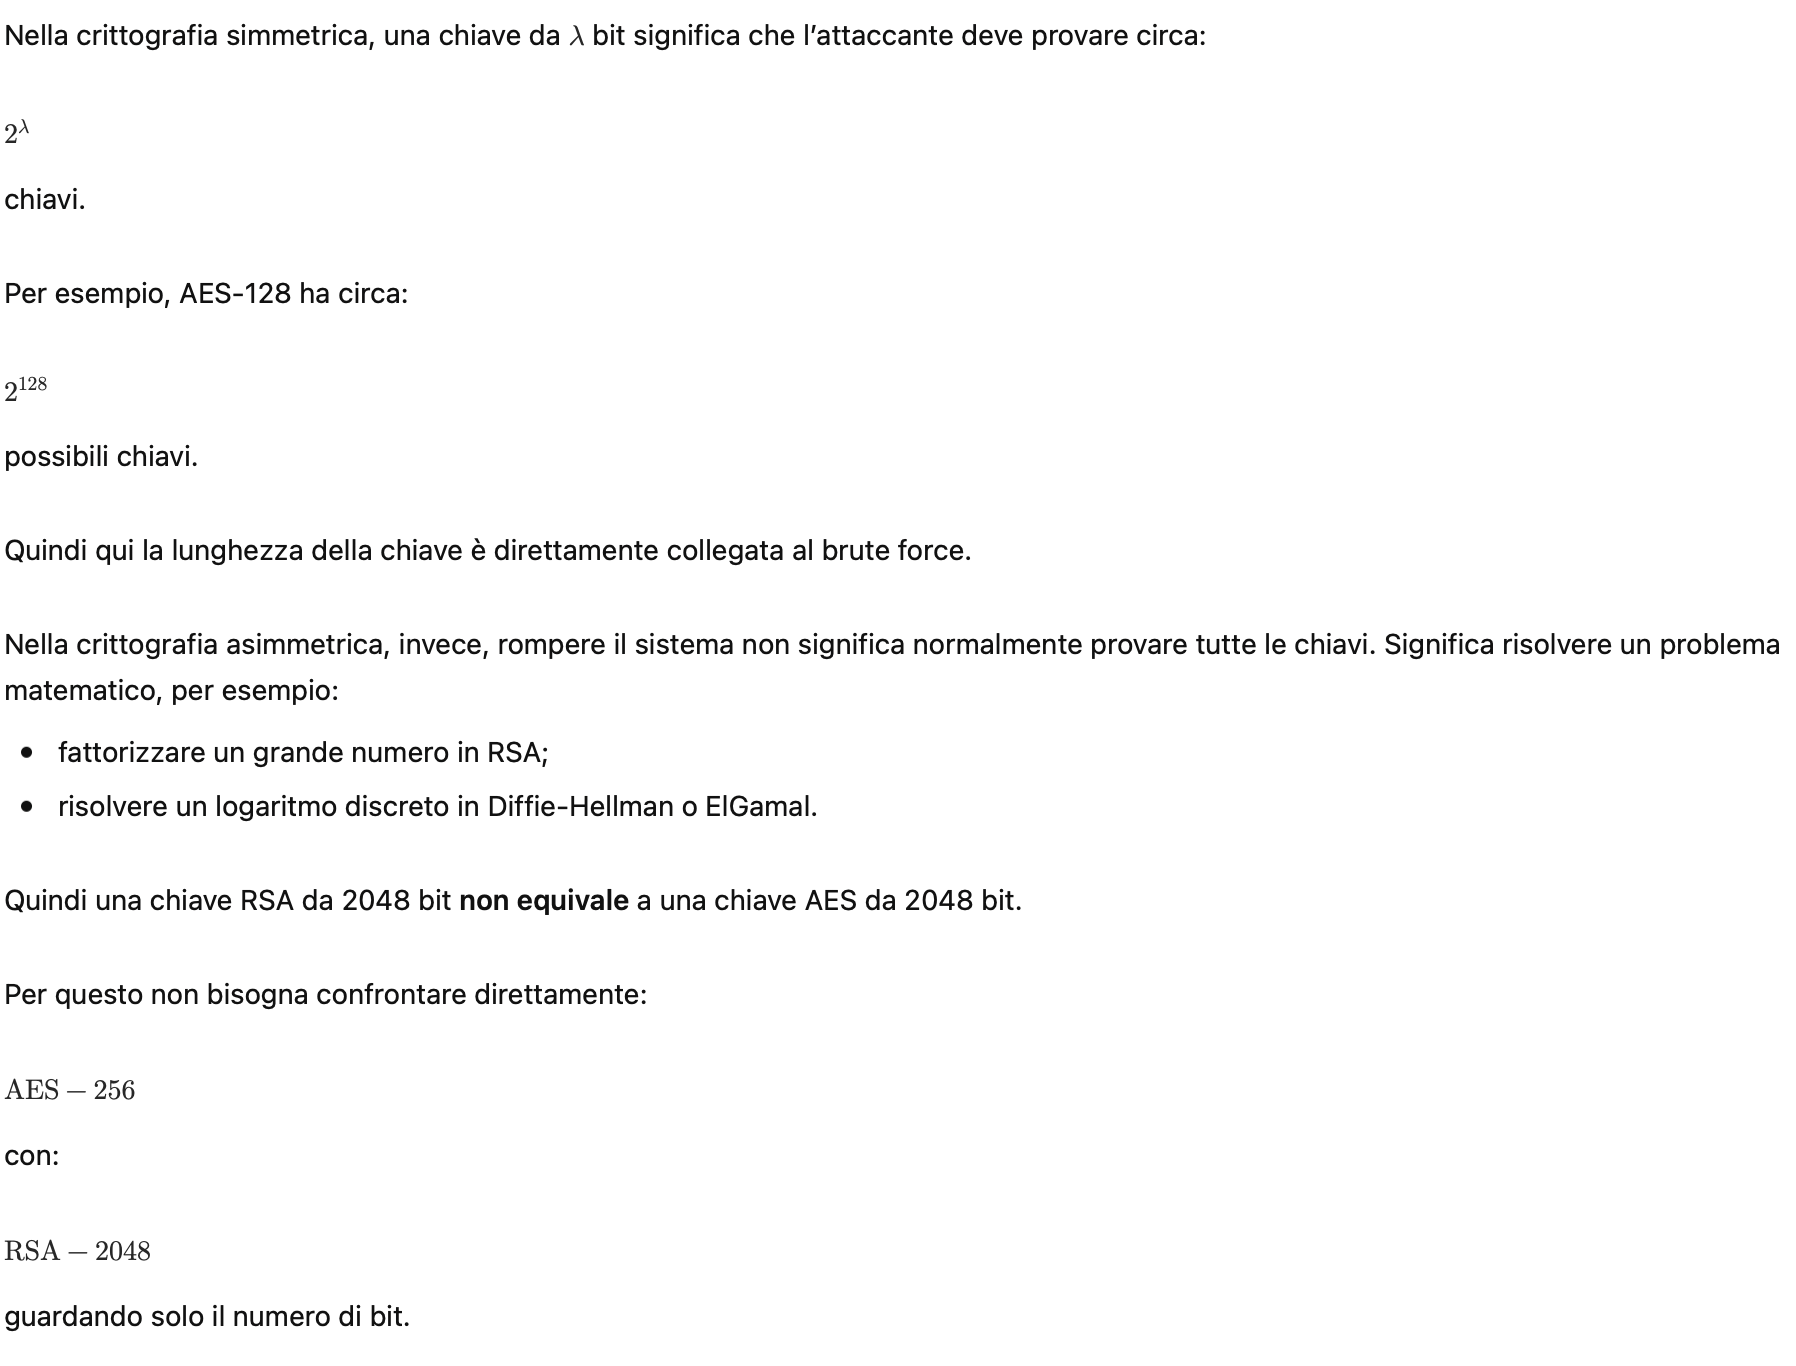
\includegraphics[width=0.8\textwidth]{media/image35.png} \end{figure}

Comparisons only make sense within the same family, for example:

AES-128 vs AES-256

or:

RSA-2048 vs RSA-4096

but not directly between symmetric and asymmetric.

\subsubsection*{Hybrid Encryption}

In theory, Bob could encrypt an entire long message using Alice's public key.

However, in practice it would be \textbf{inefficient}.

Asymmetric cryptography is much slower than symmetric cryptography. From 10 to 1000 times slower compared to symmetric schemes.

Therefore, using RSA or other asymmetric schemes to encrypt large amounts of data would be inconvenient and slow.

For this reason, in practice a \textbf{hybrid approach} is used.

Modern schemes combine asymmetric and symmetric cryptography.

The idea is:
\begin{enumerate}
\item generate a random symmetric key;
\item use this symmetric key to encrypt the real data, for example with AES;
\item encrypt only the symmetric key using the recipient's public key;
\item send:
\begin{itemize}
\item the encrypted symmetric key;
\item the ciphertext of the data.
\end{itemize}
\end{enumerate}

\begin{figure}[H] \centering 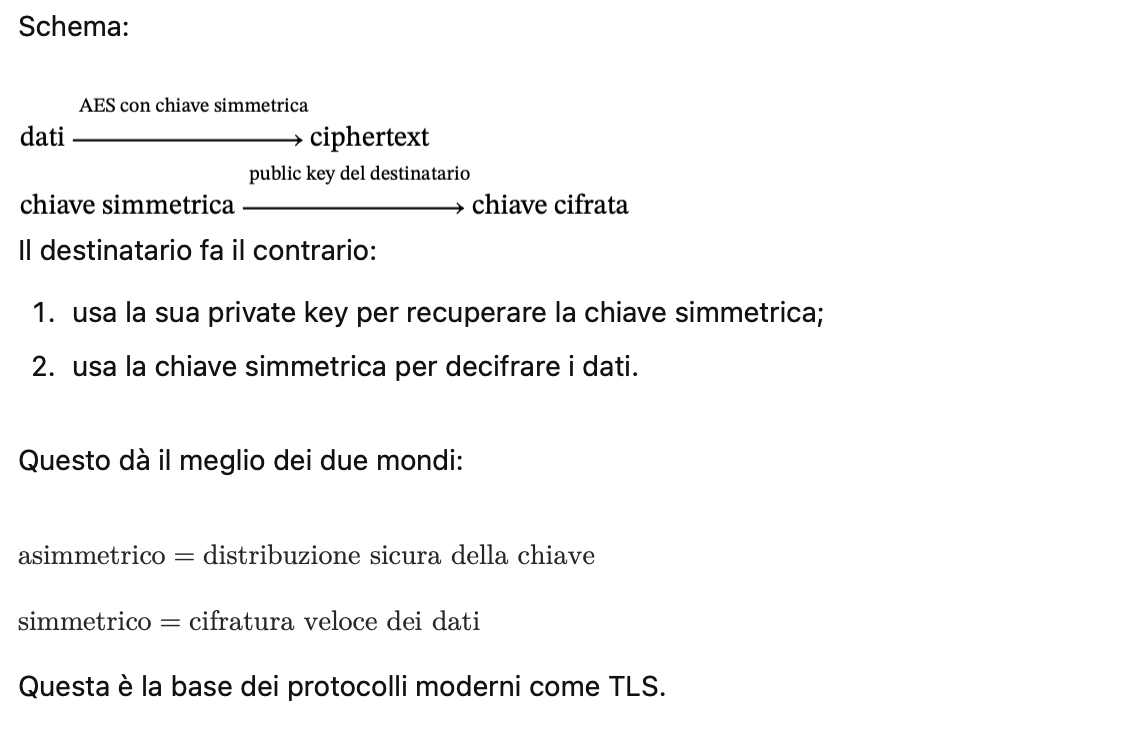
\includegraphics[width=0.8\textwidth]{media/image36.png} \end{figure}

\subsubsection*{Digital Signatures}

In hybrid encryption, however, there is an important problem.

When Bob uses Alice's public key, he must be sure that that key really belongs to Alice.

If an attacker replaces Alice's public key with their own, Bob could encrypt the symmetric key for the attacker without noticing.

So it's not enough to have confidentiality: data and public keys must also be authenticated.

Here come into play \textbf{digital signatures} and, more generally, key certification mechanisms.

\textbf{Digital signatures} are asymmetric algorithms used to authenticate data.

They work the opposite way compared to public encryption:
\begin{itemize}
\item the sender signs with their private key;
\item anyone can verify the signature with the sender's public key.
\end{itemize}

If the verification succeeds, then we have \textbf{evidence} that:
\begin{enumerate}
\item the message has not been modified;
\item the message is linked to the owner of the private key;
\item the sender cannot easily deny having signed it.
\end{enumerate}

Security requires that it is \textbf{computationally difficult}:
\begin{itemize}
\item to sign a message without the signing key;
\item to derive the signing key from the verification key;
\item to derive the signing key by observing many already signed messages;
\item to construct a valid signature by combining previously seen signatures.
\end{itemize}

This is the concept of \textbf{unforgeability}, meaning the practical impossibility of falsifying valid signatures.

In practice, \textbf{the entire message is not directly signed}, because it would be inefficient.

It is done like this:
\begin{enumerate}
\item calculate the hash of the message;
\item sign the hash with the private key;
\item send the message and the signature.
\end{enumerate}

The receiver verifies like this:
\begin{enumerate}
\item calculate again the hash of the received message;
\item use the sender's public key to verify the signature and recover/check $h$;
\item compare: $h = h'$
\end{enumerate}

If they match, the signature is valid.

This guarantees \textbf{integrity}, because if the message changes, the hash also changes. So the verification fails.

It also guarantees \textbf{authenticity}, because only the one who possesses the private key should be able to generate a valid signature.

Attention: security depends on both the signature and the hash function. If the signature is secure but the hash is broken, the entire system can become vulnerable.

\textbf{Common signature schemes: RSA and DSA}

\textbf{RSA signatures}

RSA is particular because the same mathematical idea can be used both for asymmetric encryption and for digital signatures, even though the way messages are processed is different.

An important characteristic is that in RSA signing is much slower than verification, about hundreds of times slower. This can be useful if few entities sign, but many have to verify.

\textbf{DSA}

DSA, Digital Signature Algorithm, is designed specifically for digital signatures.

In DSA, signing and verification have more similar computational costs.

\textbf{Uses of digital signatures}

Digital signatures are used to authenticate digital documents.

They are also used to authenticate users without a password.

Example:
\begin{itemize}
\item the server knows the user's public key;
\item the server sends a random challenge;
\item the client signs the challenge with their private key;
\item the server verifies the signature with the public key.
\end{itemize}

If the verification succeeds, the client has demonstrated to possess the private key.

However, this only proves that someone possesses that private key. It does not automatically prove "who" that person is, if the public key is not securely linked to an identity.

\paragraph*{Certification Authority}

\textbf{The problem of public key binding}

A valid signature says:
this message has been signed by the private key corresponding to this public key.

But it does not automatically say:

this public key truly belongs to Alice.

This is the \textbf{public key binding problem}.

The problem exists for both signatures and asymmetric encryption.

If I want to verify a signature from Alice, I must be sure that the public key I am using truly belongs to Alice.

If I want to encrypt a message for Bob, I must be sure that the public key truly belongs to Bob.

If an attacker manages to replace Bob's public key with their own, they can perform a \textbf{man-in-the-middle} attack.

So the point is:

public key $\neq$ identity

A mechanism is needed that reliably binds a pk to an identity.

The solution is to use \textbf{digital certificates}.

A digital certificate binds a public key to an identity.

This bond is signed by a trusted third party: the \textbf{Certification Authority}, or \textbf{CA}.

The CA takes:

\begin{itemize}
\item identity of the subject;
\item public key of the subject;
\end{itemize}

and signs this information with its own private key.

The certificate thus contains:

\begin{itemize}
\item identity of the subject;
\item public key of the subject;
\item identity of the issuer, i.e., the CA;
\item signature of the CA.
\end{itemize}

When Alice wants to communicate with Bob, she receives Bob's certificate and verifies the CA's signature using the CA's public key.

If the verification succeeds, Alice can trust that the public key truly belongs to Bob, assuming she trusts the CA.

\textbf{Certificate chain and root of trust}

However, a question arises:

who certifies the public key of the CA?

A CA can in turn have a certificate signed by another CA. This creates a \textbf{certificate chain}.

The problem is that this chain cannot go on indefinitely. At some point, an initial trusted element is needed.

This element is called the \textbf{root of trust}.

In the case of PKI, the root of trust is a \textbf{root CA}.

The root CA often uses a \textbf{self-signed} certificate, meaning signed by itself. This certificate cannot be verified through another higher CA: it is accepted because it is already present in the system as trusted.

Browsers and operating systems have a repository of trusted root CAs, called \textbf{trusted storage}.

So trust starts from a few pre-installed root CAs and is then delegated downwards through signed certificates.

\textbf{Hierarchy of CAs}

The structure of CAs is hierarchical, similar to a tree.

At the top is the \textbf{root CA}.

Below are the \textbf{intermediate CAs}, whose certificates are signed by the root CA.

At the bottom are the \textbf{end entities}, for example websites or users, whose certificates are signed by an intermediate CA.

It is a hierarchy because it is not a single linear chain: a root CA can sign many intermediate CAs, and each intermediate CA can sign many end certificates.

\textbf{Verification of a certificate}

To correctly verify a certificate, several things must be checked.

\begin{enumerate}
\item First, \textbf{verify} that the \textbf{signature} on the document or certificate is \textbf{valid}.
\item Then, \textbf{check} that the \textbf{public key} \textbf{used} is \textbf{actually the one contained in the certificate}.
\item Next, \textbf{verify} that the \textbf{certificate} \textbf{truly belongs} to the \textbf{correct} \textbf{subject}, for example by checking the name, the Distinguished Name, or the domain.
\item Then, \textbf{verify} that the \textbf{certificate} was \textbf{signed} by a \textbf{valid CA}.
\item Then, \textbf{verify} the entire \textbf{chain up to the root} CA.
\item Then, \textbf{check} that the \textbf{root} CA \textbf{is} \textbf{among} those \textbf{trusted} \textbf{by the system}.
\item Finally, \textbf{check} that the \textbf{certificate} has \textbf{not} been \textbf{revoked}.
\end{enumerate}

If any of these checks are missing, there may be a vulnerability.

\textbf{Certificate Revocation}

Even though a digital signature cannot be ``cancelled'' in the classical sense, a certificate can become no longer reliable.

For example, if the private key associated with a certificate is compromised, that certificate must be revoked.

We have \textbf{two main mechanisms}:

\textbf{CRL}, which is \textbf{Certificate Revocation List}, a periodic list of revoked certificates.

\textbf{OCSP}, which is \textbf{Online Certificate Status Protocol}, which allows checking the validity status of a certificate online in real time.

OCSP is generally more up-to-date and efficient compared to CRLs.

\textbf{Attacks and limitations of digital signatures}

Digital signatures are more secure than written signatures, because a digital signature is mathematically bound to the content.

If the document changes, the signature is no longer valid.

However, they are not ``magic''. If the signature algorithm or the hash function is broken, the signature can be forged.

Furthermore, a digital signature is fragile: if a forgery is produced correctly, it can be indistinguishable from a real signature.

Therefore, the entire security depends on:

\begin{itemize}
\item signature algorithm;
\item hash function;
\item protection of the private key;
\item correct binding between public key and identity;
\item correct verification of the certificate chain.
\end{itemize}

\textbf{Putting it all together}

The last slide puts together all the pieces of modern secure communication.

On the left is the CA:

\begin{itemize}
\item takes the identity and public key of the recipient;
\item signs this information with the CA's private key;
\item produces a certificate.
\end{itemize}

This solves the problem of binding between identity and public key.

On the right is the sender:

\begin{enumerate}
\item obtains and verifies the recipient's certificate;
\item extracts the recipient's public key;
\item generates a random symmetric key;
\item encrypts this symmetric key with the recipient's public key;
\item encrypts the actual message with the symmetric key;
\item sends:
\begin{itemize}
\item encrypted symmetric key;
\item ciphertext of the message.
\end{itemize}
\end{enumerate}

This is a scheme of \textbf{hybrid encryption}.

Asymmetric cryptography is used to protect/exchange the key.\\
Symmetric cryptography is used to efficiently encrypt the data.

This approach is the basis of modern protocols such as:

TLS/HTTPS,\\ OpenVPN,\\ IPsec

\begin{figure}[H]
\centering
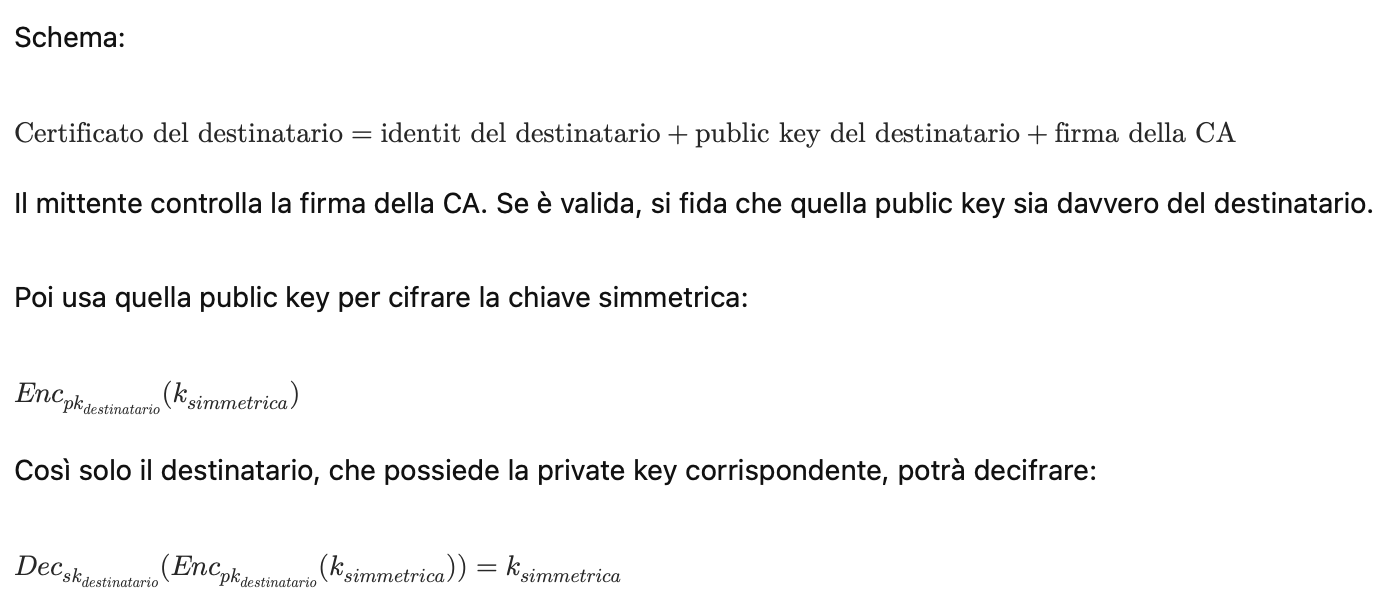
\includegraphics[width=0.8\textwidth]{media/image38.png}
\end{figure}

\section{Binary Exploitation}

When analysing a binary for exploitation, a \textbf{disassembler} is used to translate machine code to assembly code and a \textbf{decompiler} tries to reconstruct a high-level representation of the program. The final reconstruction is always lossy, in particular due to compiler optimization. This makes \textbf{binary reconstruction more challenging} as understanding the program's behaviour requires interpreting incomplete or transformed information.

\begin{figure}[H]
\centering
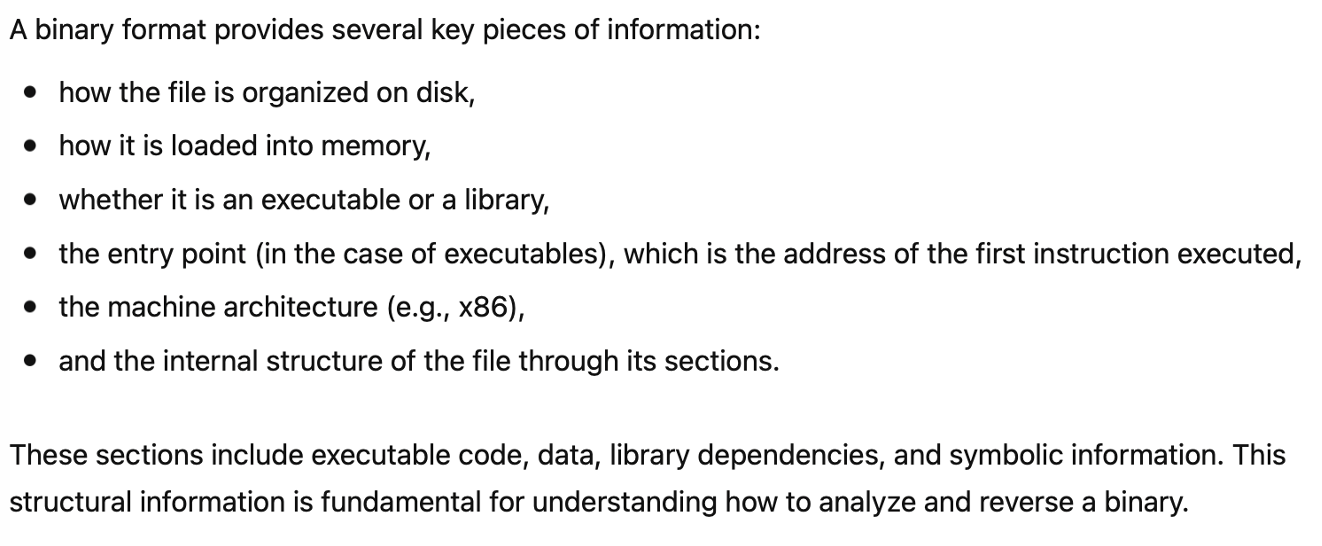
\includegraphics[width=0.8\textwidth]{media/image39.png}
\end{figure}

\textbf{ELF binaries} (commonly used on Linux systems) are organized into several components:

\begin{itemize}
\item \textbf{ELF} header: describes the overall structure of the binary, defining the file type and the section and program headers boundaries.
\item \textbf{Program Headers}: describe how the file will be loaded in memory. It divides the data into segments and map sections to segments.
\item \textbf{Segments}: runtime view of the ELF.
\item \textbf{Sections}: linking and relocation information.
\begin{itemize}
\item \textbf{Sections} are primarily used for linking and organizing the binary on disk, while \textbf{segments} represent how these sections are grouped and loaded into memory at runtime.
\end{itemize}
\item \textbf{Section Headers}: Define the sections
\begin{itemize}
\item \begin{figure}[H]
\centering
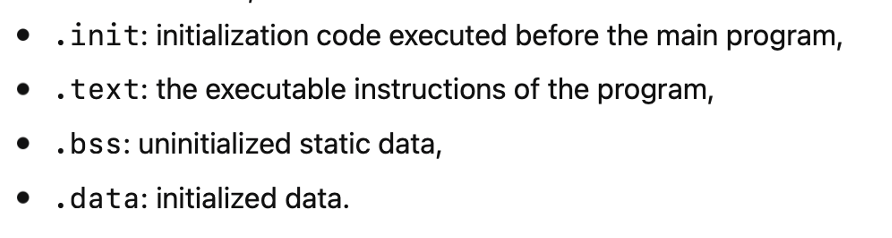
\includegraphics[width=0.8\textwidth]{media/image40.png}
\end{figure}
\item By inspecting the section headers, \textbf{it is possible to locate precisely where each part of the binary is on disk}.
\end{itemize}
\end{itemize}

When analysing a binary file, the first element to consider is the \textbf{magic number} which is a sequence of bytes that identifies the format, for ELF binaries is 7f 45 4c 46.

The ELF header contains information about the \textbf{offsets and sizes} of the \textbf{program} and \textbf{section} \textbf{headers}, and (if the file is an executable) also the \textbf{entry point address} which is the memory address of the first instruction to execute.

By analysing the \textbf{program header}, it is possible to understand how the binary is mapped into memory at runtime. In particular, the program header shows the relationship between \textbf{sections} and \textbf{segments}.

\textbf{Section header} instead provides a more disk level view of the binary. For each section is possible to determine whether it is:

\begin{itemize}
\item \textbf{Writable} (can be modified at runtime)
\item \textbf{Allocatable} (will be loaded into memory)
\item \textbf{Executable} (contains instructions that the CPU can execute)
\end{itemize}

\textbf{Executing a program}

When a program is executed, it is \textbf{mapped into memory} in a structured and organized way.

Then, the kernel creates a \textbf{virtual address space} in which the program runs. This space is divided into \textbf{user space} (where user-level processes are executed) and \textbf{kernel space} (where OS-level processes are executed).

A user process cannot directly access kernel space to execute privileged instructions. Instead, it must rely on \textbf{system calls}, which trigger an interrupt handled by the kernel. The kernel executes the requested operation and then returns control to user space. This separation enforces security and isolation between user processes and the operating system.

Then, the system loads the content into memory. This is done by the \textbf{dynamic} linker which loads the segments \textbf{defined by the program headers}.

Finally, the kernel sets up two essential memory regions: the \textbf{stack} and the \textbf{heap}. Once these are initialized, the execution of the program begins by transferring control to the \textbf{entry point} specified in the binary.

The \textbf{stack} and the \textbf{heap} are two memory regions used differently during program execution.

The \textbf{stack} stores the execution context of a process, including local variables and function activation records. Each function call adds information to the stack. The stack grows from \textbf{higher memory addresses to lower memory addresses}.

Because it contains important control-flow information, it is a common target for attacks such as \textbf{stack smashing}, where an attacker tries to overwrite critical stack data through a buffer overflow.

The \textbf{heap}, instead, is used for \textbf{dynamic memory allocation}, such as memory allocated at runtime with malloc in C.

Unlike the stack, the heap grows from \textbf{lower memory addresses to higher memory addresses}.

Although exploitation often focuses on the stack, heap-based attacks also exist and target dynamically allocated memory.

Finally, the \textbf{.text section} contains the program's executable machine code. The CPU fetches and executes instructions from this section, while the effects of those instructions, such as function calls and variable handling, are reflected mainly in the stack.

\begin{figure}[H]
\centering
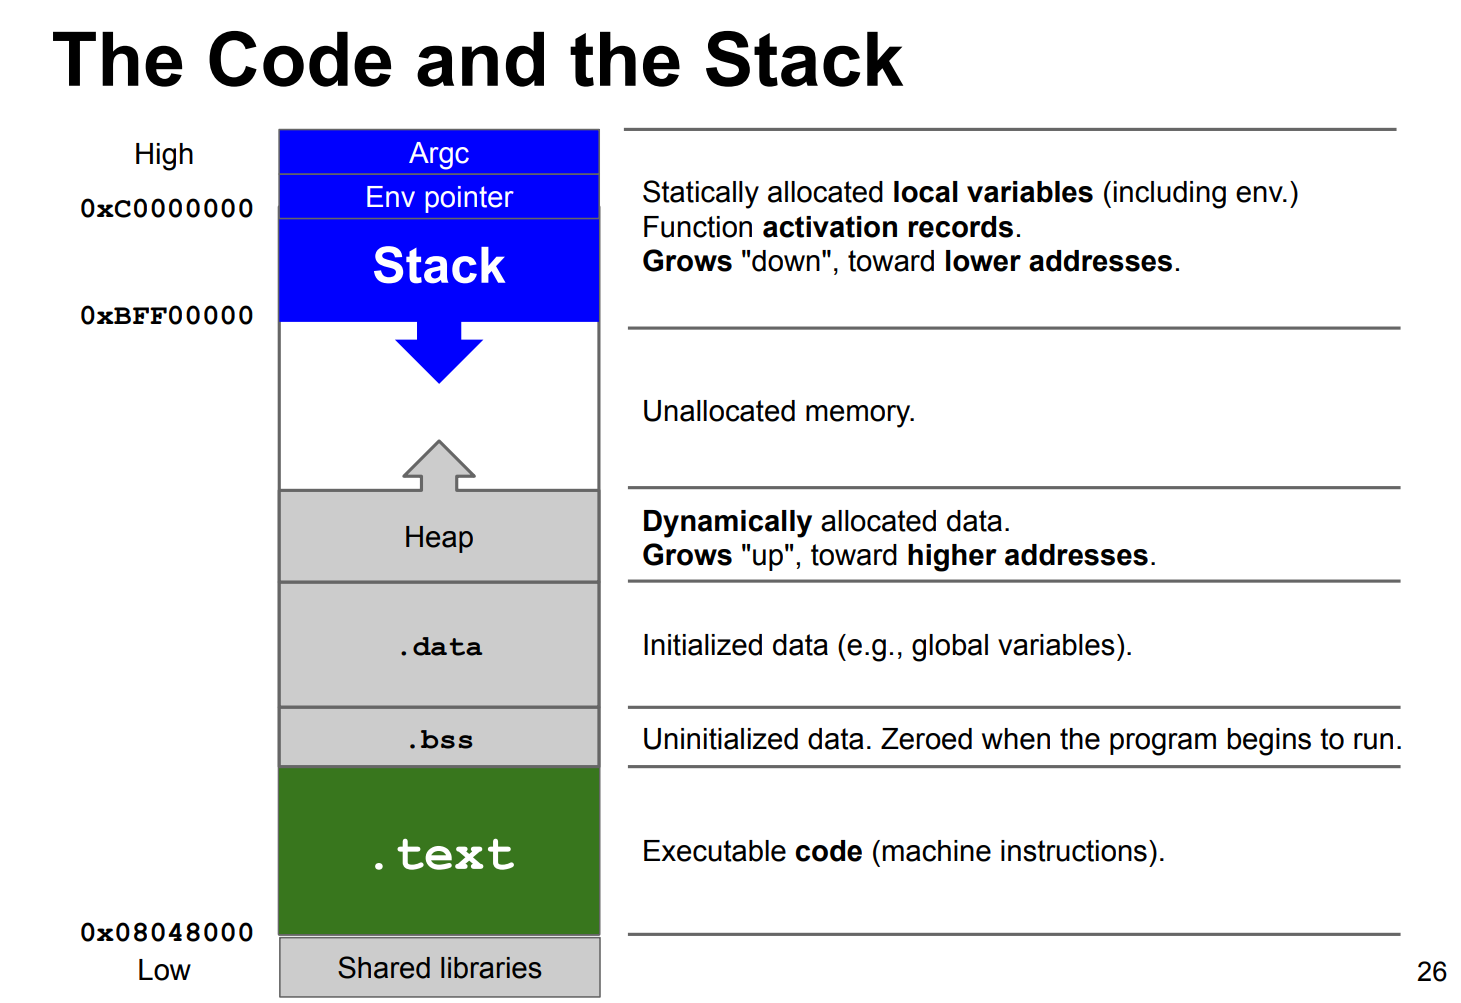
\includegraphics[width=0.8\textwidth]{media/image41.png}
\end{figure}

The stack is manipulated through two fundamental instructions:

\begin{figure}[H]
\centering
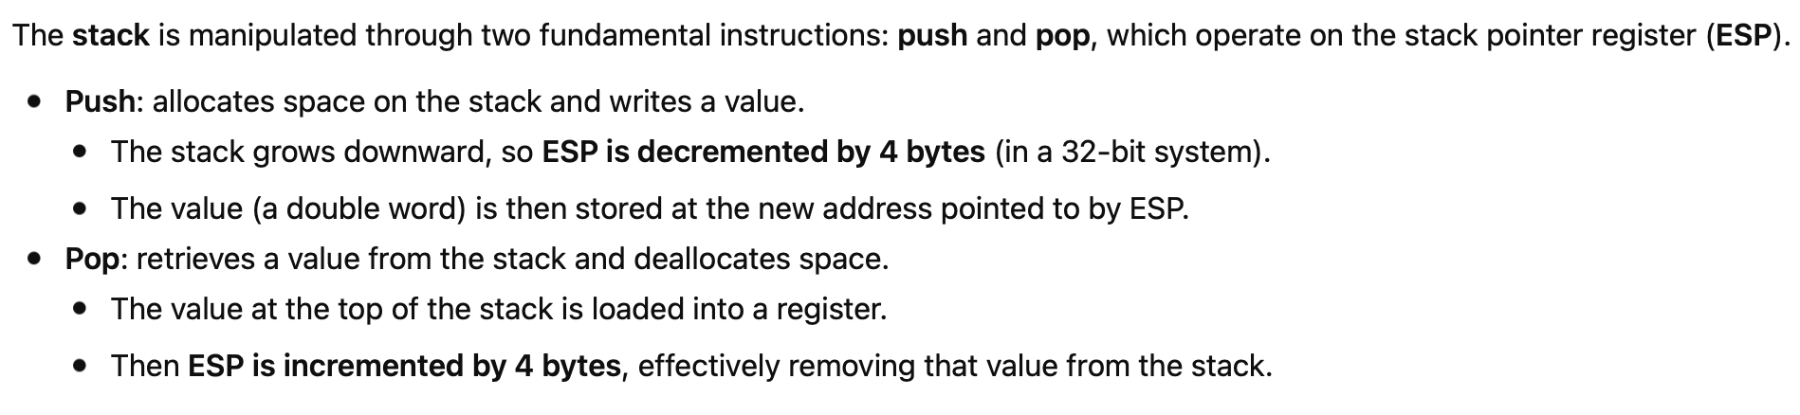
\includegraphics[width=0.8\textwidth]{media/image42.png}
\end{figure}

The \textbf{ESP register} stores the addres of the \textbf{top of the stack} (last stack operation).

The \textbf{EIP register} stores the address of the next machine instruction to be executed.

When the binary is executed, the CPU begins execution at the \textbf{entry point} inside the .text section, which contains the executable instructions. Execution proceeds sequentially from lower to higher memory addresses.

At some point, control reaches the \textbf{main function}, which is entered through a jump in the instruction flow.

\begin{figure}[H]
\centering
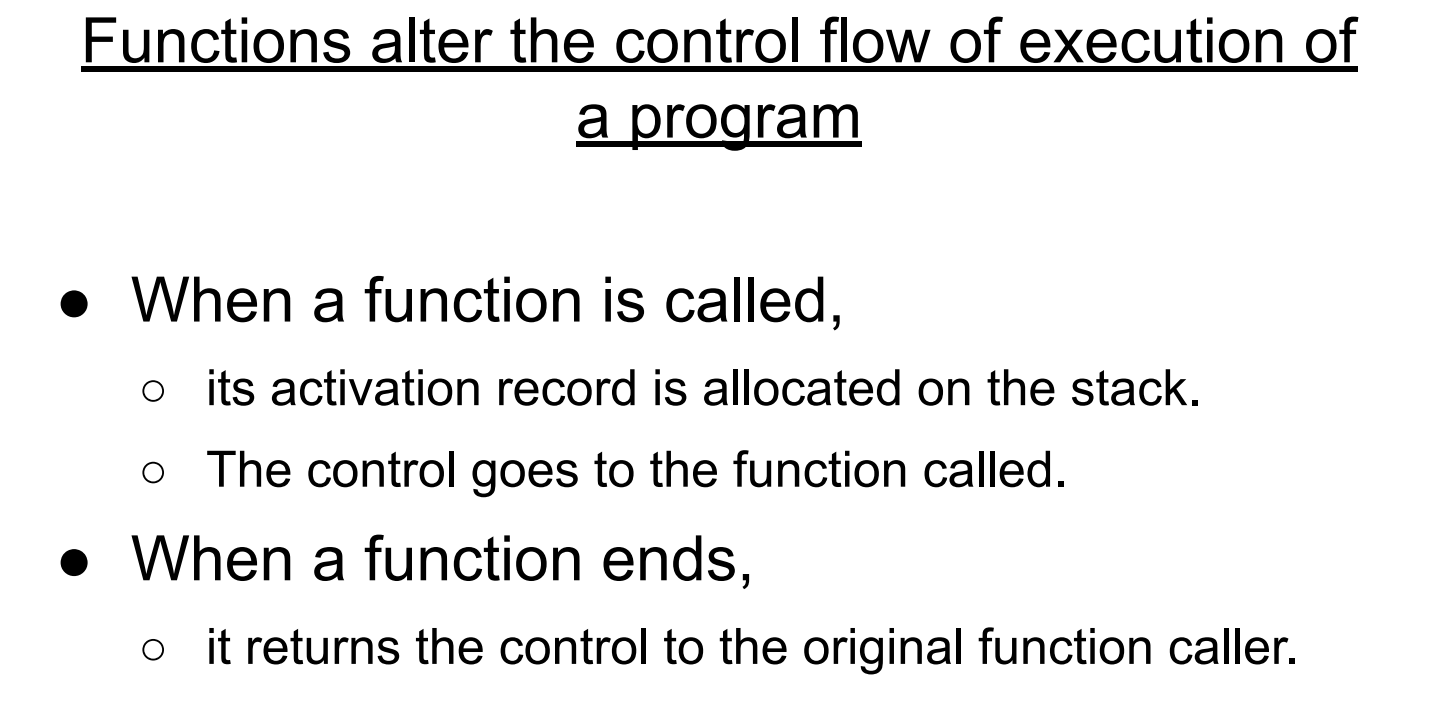
\includegraphics[width=0.8\textwidth]{media/image43.png}
\end{figure}

When a function is called, before the control passes to the called function, the caller places the arguments on the stack in \textbf{reverse order}.

These arguments are \textbf{passed by value}, meaning that the called function receives copies of the argument values. Therefore, if the function modifies a parameter, it modifies only its own copy, not the original variable in the caller.

After the paramaters are saved onto the stack, the call instruction is executed.

The \textbf{call} instruction \textbf{performs two operations}:

\begin{enumerate}
\item \textbf{Pushes} the \textbf{current EIP} (the addres of the instruction where execution must continue after the function ends) onto the stack.
\item \textbf{Jumps} to the \textbf{address of entry point of the called function}.
\end{enumerate}

At this point, the called function begins executing, but it first needs to create its own stack frame. This initial phase is called the \textbf{function prologue}.

During this phase the \textbf{base pointer EPB} value is saved onto the stack, and then it is updated so that it points to the \textbf{called function frame}.

(The base pointer, \textbf{EBP}, identifies the base of the current stack frame.)

When the function finishes, the \textbf{function epilogue} is executed. The called function stack frame is removed, the \textbf{frame of the caller} \textbf{is} \textbf{restored} thanks to the EPB value saved on the stack and the EIP is used to resume the execution of the caller.

\begin{quote}
When a function is executing, its \textbf{stack frame already exists on the stack}. It contains its parameters, its local variables, the return address, saved registers, etc.

When this function calls another function, its frame \textbf{remains on the stack}, but the execution passes to the called function. On top of the caller's frame, a new frame is built, which is the \textbf{callee's frame}.
\end{quote}

However, if the return address stored on the stack is \textbf{modified}, the program \textbf{does not return} to the original caller \textbf{correctly}.

When a function finishes, the CPU retrieves the saved return address from the stack and uses it to decide where execution must continue. The CPU does not check whether that address is legitimate; it simply loads it and jumps to it.

Therefore, if an \textbf{attacker} manages to \textbf{overwrite the return address}, the \textbf{control flow} of the program \textbf{can be redirected} to another location.

This is the basic idea behind \textbf{stack smashing}, also known as a \textbf{stack-based buffer overflow attack}.

\textbf{The attack usually occurs} when a function allocates a buffer on the stack and then writes data into it without checking the size of the input. If the input is larger than the buffer, the extra data goes beyond the buffer boundaries and overwrites adjacent stack data.

If the overflow reaches the return address, the attacker can replace it with another value. When the function later returns, the corrupted return address is used.

This vulnerability is especially associated with unsafe C functions that do not automatically enforce bounds checking.

If the programmer does not validate the input size, a \textbf{buffer overflow} can occur.

\subsection{Buffer Overflows}

A buffer overflow becomes exploitable only \textbf{under specific conditions}.

The \textbf{basic condition} is that the program writes more data into a buffer than the buffer can contain, without checking the input size.

This happens because the buffer is stored on the stack together with other data.

The \textbf{stack} grows from higher addresses to lower addresses,

but \textbf{data written into a buffer} is normally written from lower addresses to higher addresses.

Therefore, if the input is longer than the buffer, the program continues writing beyond the buffer boundary.

The \textbf{first values overwritten} are usually \textbf{nearby local variables}.

\textit{This can already be dangerous. For example, if a local variable stores the result of a security check, changing that variable may alter the program's behavior without even reaching the return address.}

If the overflow continues, it \textbf{may overwrite the saved base pointer}. This can \textbf{affect how the previous stack frame is restored} during the function epilogue.

If the overflow reaches the saved \textbf{return address} and overwrites it, the program no longer returns to the correct instruction. Instead, it \textbf{jumps to the address placed there by the input.}

\textbf{At first}, this usually causes a crash, such as a segmentation fault, because the overwritten return address \textbf{may contain meaningless bytes} that do not correspond to a valid memory address. However, the crash is still important because \textbf{it proves that the input can influence the program's control flow}.

To turn the crash into a real exploit, \textbf{the attacker would need to replace the invalid address with a valid memory location} that leads to executable code or to useful existing code inside the program.

That is the step that transforms a simple overflow into control of the program.

So, a buffer overflow can affect the program in different ways:

\begin{enumerate}
\item it can overwrite local variables,
\item corrupt the saved base pointer,
\item overwrite the saved return address (the most dangerous case).
\end{enumerate}

The \textbf{main conditions} required for a buffer overflow are the following:

\begin{enumerate}
\item A program allocates a buffer.
\item The program does not perform proper bounds checking on the input
\begin{itemize}
\item In this way, the excess data overflows the buffer and overwrites adjacent memory locations, hence the attacker can craft data to inject in some locations.
\end{itemize}
\item CPU does not inherently distinguish between code and data.
\begin{itemize}
\item In this way, the processor executes whatever is injected into
\end{itemize}
\end{enumerate}
memory.

\begin{enumerate}
\setcounter{enumi}{3}
\item \underline{Memory is allocated in one direction and written in the opposite one}.
\end{enumerate}

\underline{The aim of the attaccker} is to \textbf{redirect execution toward a memory location containing executable code that can actually be executed and controlled by him/her}.

\subsection{Address Problem}

From an attacker's perspective, the first major challenge is to \textbf{make the program jump wherever he/her want}.

There are different possible locations where execution may be redirected:

\begin{enumerate}
\item One possibility is to jump to a \textbf{memory location that the attacker can control indirectly}. These are typically variables that can be influenced through the program itself, for example global variables or memory areas containing user-controlled information such as environment variables.

\item Another possibility is \textbf{to jump directly to an already existing function}.

\item The third option is to \textbf{jump in memory that can control}, hence, to \textbf{jump inside the buffer itself} since it is controlled by the attacker through the program's input. Therefore, if execution can be redirected into the buffer, the attacker gains control over the sequence of bytes that the CPU will interpret and execute.
\end{enumerate}

To \textbf{make the overflow exploitable}, the overwritten return address must point to a valid memory location. In the classical stack-smashing model, this region is the buffer itself, hence \textbf{the input contains both executable bytes and the address that redirects execution back into the buffer}.

\underline{The key idea is that the CPU does not distinguish between "normal data" and "instructions" by itself}

If execution is redirected to a memory region and that region is executable, the CPU will interpret the bytes found there as machine instructions.

This creates \textbf{two main practical problems}.:

First, there must be \textbf{enough space} \textbf{in the buffer} to contain 1. the required payload and 2. the overwritten control data.

Second, \textbf{the attacker must know where the buffer is located in memory}. The overwritten return address must be precise. Even a small error can make the program jump to the wrong location or into the middle of an instruction, causing another crash.

\begin{figure}[H] \centering 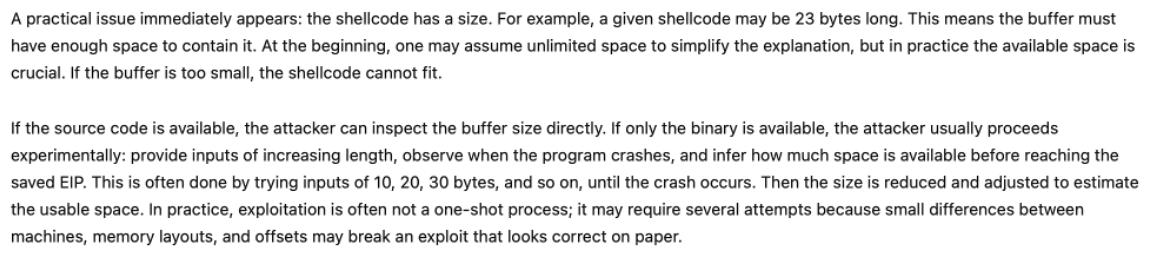
\includegraphics[width=0.8\textwidth]{media/image44.png} \end{figure}

The attacker may try to estimate the position of the buffer by reading the value of the \textbf{ESP register}. Since ESP points to the top of the stack, it gives an approximate indication of where the local variables of the current function are located, including the vulnerable buffer.

One possible way to obtain this value is to use a debugger such as \textbf{GDB}. In GDB, the attacker can inspect the current value of ESP and use it as a reference point to estimate the address of the buffer.

\underline{\textbf{However}, some debuggers, including GDB, can \textbf{add an offset}. Therefore, the ESP value obtained through GDB may differ by a few words from the real value during normal execution.}

For this reason, \textbf{another possibility} is to \textbf{read the value of ESP directly from inside the process} itself. This may give a more accurate value for that specific execution.

In both cases, the main problem remains \textbf{precision}. Even if the attacker obtains an approximate stack address, the jump address must be accurate enough to land inside a valid instruction sequence. If execution lands in the wrong place, the program will likely crash.

To reduce this precision problem, attackers historically used a \textbf{NOP sled}. A NOP instruction is a one-byte instruction that means "no operation": the CPU does nothing and simply moves to the next instruction.

\underline{If a memory region is filled with many NOP instructions, execution can land anywhere inside that region and still continue safely until it reaches the actual payload}

So, instead of needing to jump to the exact first byte of the code, \textbf{it is enough to jump somewhere inside the NOP sled}.

\begin{figure}[H] \centering 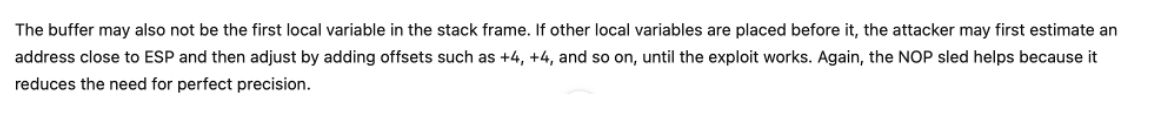
\includegraphics[width=0.8\textwidth]{media/image45.png} \end{figure}

\subsection{What to Execute}

Once the attacker knows the address, the second problem is deciding \textbf{what to execute} after the jump.

The code placed inside the buffer is called \textbf{shellcode}. Shellcode is not high-level source code; it is a sequence of machine instructions that the CPU can execute directly.

The goal was often to \textbf{spawn a shell}, but in general shellcode can perform different actions such as open a shell as mentioned, open a TCP connection, execute a command, etc.

\begin{figure}[H] \centering 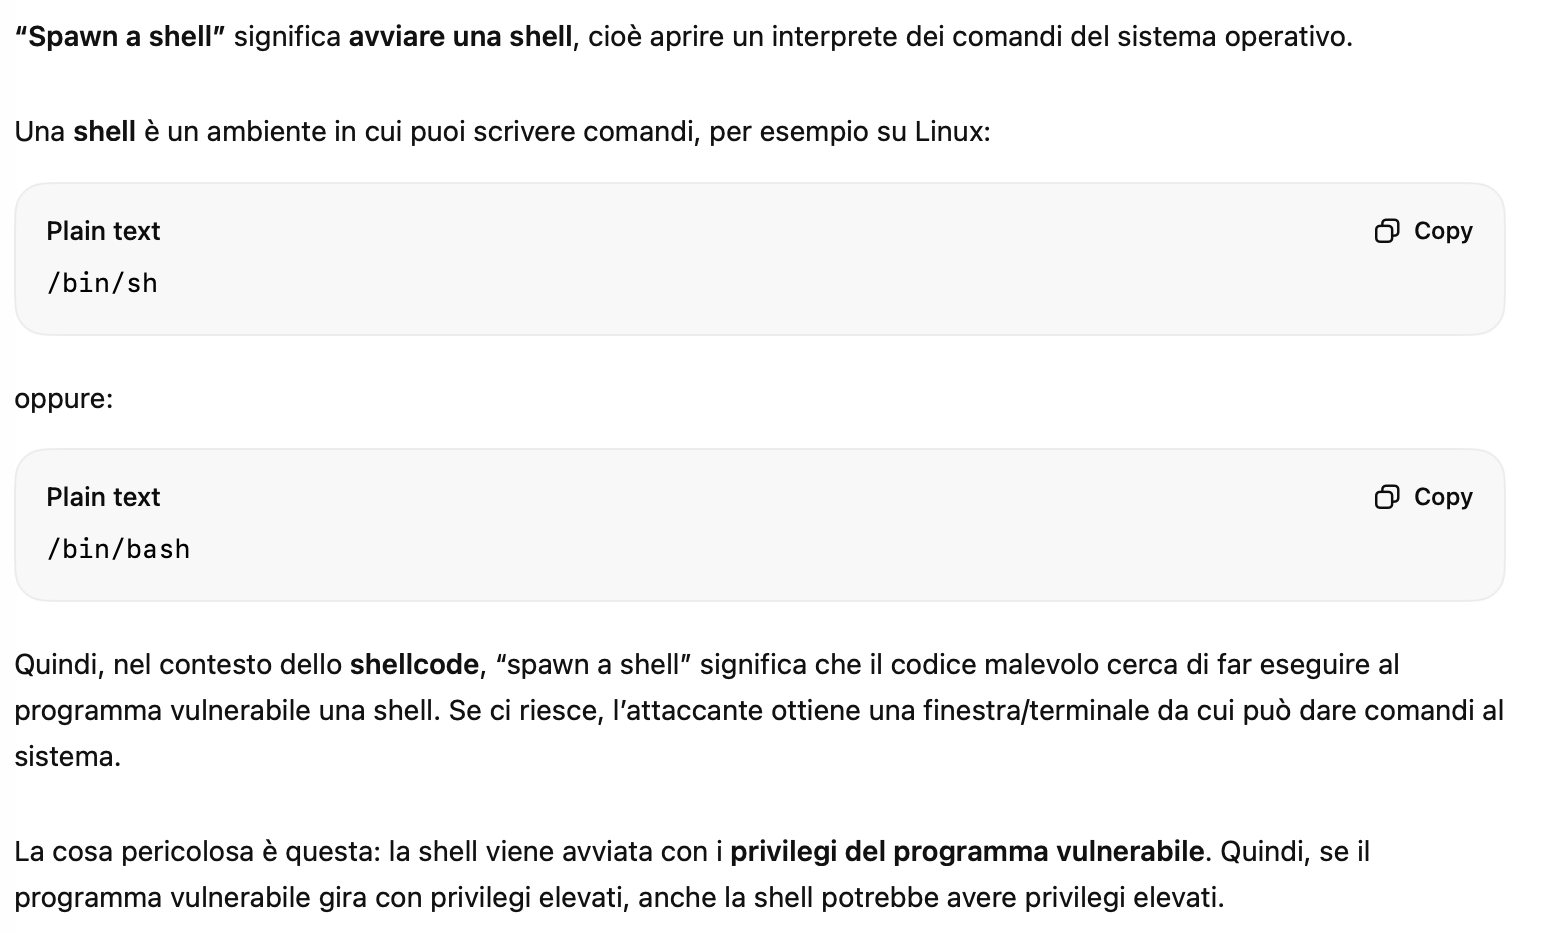
\includegraphics[width=0.8\textwidth]{media/image46.png} \end{figure}

If the shell is spawned, it \textbf{will run with priviliges of the vulnerable program}.

The \textbf{exploit payload} therefore has \textbf{three conceptual parts}:

\begin{enumerate}
\item first a NOP sled,
\item then the shellcode,
\item and finally the overwritten return address that redirects execution back into the buffer.
\end{enumerate}

\subsection{How to build the Shellcode}

At this point, the attacker already knows approximately \textbf{where to jump} and \textbf{what kind of code should be executed}. The next problem is how to build the shellcode.

\textbf{A first simple idea} is to \textbf{write a small C program that performs the desired action}, compile it, disassemble it, and extract the machine instructions.

However, this approach has a problem: the generated code may contain fixed memory addresses. If the shellcode is moved to another execution context, \textbf{those addresses may no longer be valid}, and the shellcode will fail.

For this reason, shellcode should be \textbf{portable}. This means that it should not depend on hard-coded addresses. Instead, it should build the memory structure it needs at runtime.

In the classical example, the goal of the shellcode is to \textbf{execute /bin/sh}, that is, to start a shell.

However, writing /bin/sh inside the buffer is not enough, because \textbf{/bin/sh is only a string}, not executable code.

To actually execute /bin/sh, \textbf{the shellcode must invoke the appropriate system call}, which needs \textbf{the address of the string /bin/sh}

So, the \textbf{buffer must contain two different things}:

First, it must contain the \textbf{shellcode}, which is executable machine code. This code prepares the system call and asks the operating system to execute /bin/sh.

Second, it must contain the \textbf{string /bin/sh}, which is data used by the shellcode. The string must also be terminated correctly with a null byte, because the operating system expects a properly terminated string.

The main problem is that \textbf{the shellcode needs to know where the string /bin/sh is located in memory}. It is not enough for the string to be present in the buffer; the shellcode must also pass its address to the system call.

This is \textbf{difficult} because the buffer may be loaded at \textbf{different memory addresses in different executions}. Therefore, the shellcode should not depend on fixed addresses.

To solve this problem, shellcode can use the \textbf{jump-and-call trick}. This technique uses the \textbf{behavior of the call instruction}.

When call is executed, the CPU automatically saves on the stack the address of the instruction immediately after the call. The trick is to \textbf{place the string /bin/sh immediately after the call}.

The jump-and-call trick is used to find the string's address at runtime, so the shellcode can work without relying on fixed memory addresses.

\subsubsection{Null Bytes}

Another practical problem is that \textbf{shellcode may contain 0x00 bytes}. This is dangerous because 0x00 is the string terminator in C.

\begin{figure}[H] \centering 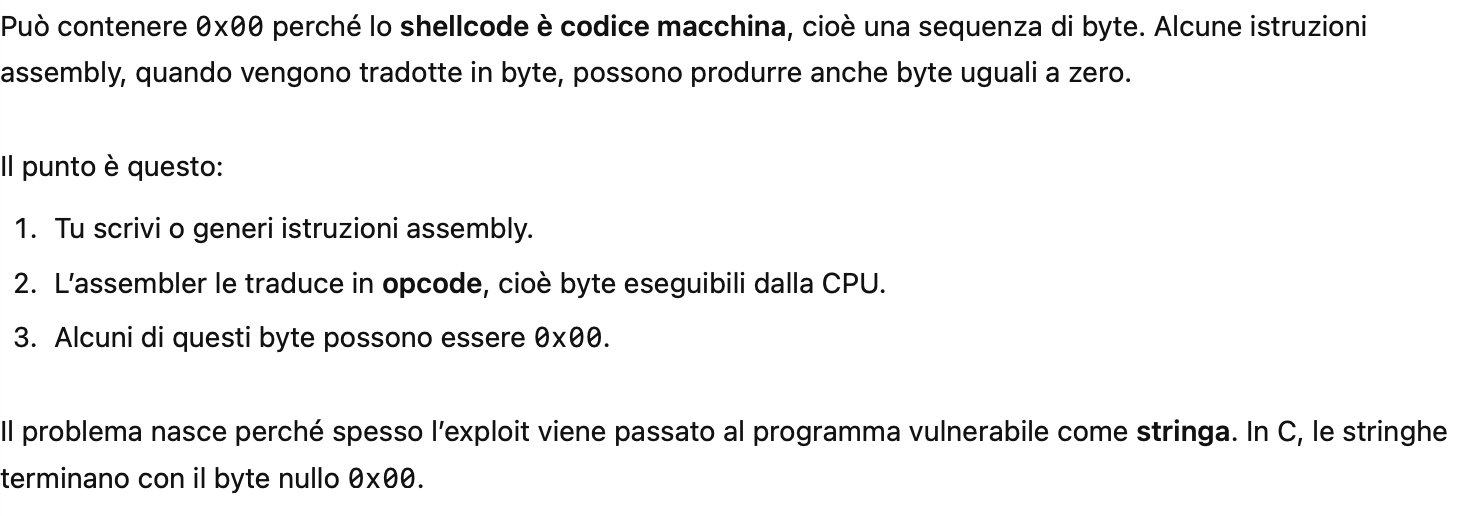
\includegraphics[width=0.8\textwidth]{media/image47.png} \end{figure}

If the exploit is passed as a string input, the vulnerable function may \textbf{stop reading as soon as it reaches the first 0x00 byte}. As a result, the shellcode would be cut off before it is fully copied into the buffer, and it would not execute correctly.

For this reason, \textbf{shellcode must be written in a way that avoids null bytes}.

Instructions that produce 0x00 in their byte representation are replaced with equivalent instructions that \textbf{achieve the same result without introducing zero bytes}.

For example, instead of directly loading a value that would contain zero bytes, the shellcode can \textbf{compute that value at runtime}.

Another example is that a register can be cleared using an operation such as XOR, and then adjusted step by step. First it clears a register using XOR, then it builds the required value with small successive operations, such as increments or additions.

The \textbf{goal} is \underline{not to change the logic of the shellcode, but to encode it in a form that can safely pass through string-based input functions}.

\subsection{Environment Variables Exploitation}

A second technique is to place the exploit inside an \textbf{environment variable} instead of placing it directly inside the vulnerable buffer.

Environment variables are values passed to a program when it starts. They are stored in the process memory, usually near the upper part of the stack. This makes them useful in this context because \textbf{their position can often be estimated more easily} than the exact position of a small local buffer.

This method works \textbf{only if the attacker has local access} to the machine.

The idea is \textbf{divided into two steps}.

First, the attacker creates an environment variable that contains the exploit payload. This payload contains the \textbf{NOP sled} and the \textbf{shellcode}.

Second, the attacker \textbf{overflows the vulnerable buffer}. This time, the goal is not to put the whole shellcode inside the buffer. The \textbf{goal} is only to overwrite the saved return address with an \textbf{address that points to the environment variable}.

When the function returns, the CPU uses the overwritten return address and jumps to the environment variable.

This \textbf{technique is easier} because \textbf{the buffer does not need to contain the whole payload}. It only needs enough input to reach and overwrite the saved return address. The larger payload is stored separately in the environment variable.

One of the problems to solve is finding \textbf{where the environment variable is located in memory}.

Environment variables are stored in the process memory, usually in the upper part of the stack. A debugger such as \textbf{GDB} can be used to inspect memory around the stack pointer. By \underline{examining memory near ESP}, it is possible to find the environment variable and verify that the payload is actually present in memory.

Once the environment variable is found, the \textbf{memory will contain three parts}:

\begin{enumerate}
\item the \textbf{name of the variable}, for example EGG=;
\item the NOP sled;
\item the shellcode.
\end{enumerate}

The attacker must be careful \textbf{not to jump to the beginning of the variable}. If execution jumps to the characters of the variable name, such as E, G, G, the CPU will interpret those characters as machine instructions, and the \textbf{exploit will fail}.

For this reason, the \textbf{return address should point slightly after the beginning of the environment variable, inside the NOP sled}.

The \textbf{advantage} of this technique is that the vulnerable buffer no longer needs to contain the whole payload. The buffer only needs to be overflowed enough to overwrite the saved return address with an address that points into the environment variable.

So the \textbf{exploitation process becomes simpler}:

First, \textbf{create an environment variable} containing the NOP sled and the shellcode.

Second, \textbf{overflow the vulnerable buffer and overwrite the saved return address} with an address inside that environment variable, preferably inside the NOP sled.

\subsection{Function Exploitation}

Instead of injecting new shellcode into the buffer or into an environment variable, the \textbf{attacker redirects execution to code that already exists in memory}.

This type of technique is called a \textbf{code reuse attack}. The idea is not to execute attacker-injected code, but to reuse existing executable code already loaded in the process.

A typical example is \textbf{return-to-libc}. In this technique, the attacker redirects execution to a function from the C standard library, such as system(). The goal is to make the program behave as if it had normally called:

system("/bin/sh")

In this case, the attacker \textbf{does not need the stack to be executable}, because \textbf{the code being executed is not on the stack}. The function system() already exists in executable memory. This is the main advantage of return-to-libc compared to classical shellcode injection.

\underline{However, simply jumping to system() is not enough}

\textbf{The stack must be arranged as if system() had been called normally}. This means that the stack must contain:

\begin{enumerate}
\item the address of system(), used to \textbf{overwrite the saved return address};
\item a \textbf{fake return address} for system(), often the address of exit(), so that the program can terminate cleanly after system() finishes;
\item the address of the string "/bin/sh", because system() needs this string as its argument.
\end{enumerate}

So the attacker \textbf{must still place the string "/bin/sh" somewhere in memory}. It may be inside the buffer, inside an environment variable, or already present somewhere in the process memory. What matters is that system() receives the correct address of that string.

When the \textbf{vulnerable function returns}, \textbf{it does not return to its original caller}. Instead, it jumps to system(). Then system() reads its argument from the stack, finds the address of "/bin/sh", and executes it. When system() finishes, execution continues to the fake return address, commonly exit().

Sometimes the \textbf{string is written as "////bin/sh" instead of "/bin/sh".} The extra slashes act like an offset.

The key point is that \textbf{return-to-libc avoids injecting new executable code}. It abuses the normal return mechanism to redirect execution to an existing library function, with the stack prepared so that the function receives valid arguments.

\subsection{Defences}

Defenses can be divided into three main levels: \textbf{source-code level}, \textbf{compiler level}, and \textbf{operating-system level}.

\subsubsection{Source-Code Level Defence}

At the \textbf{source-code level}, the main goal is to remove the vulnerability \textbf{before the program is compiled}.

Buffer overflows are usually caused by programmer mistakes, especially when input size is not checked. For this reason, \underline{programmers must validate input lengths and avoid unsafe functions}.

This can be obtained by using \textbf{safer library functions} or \textbf{languages that manage memory more safely}, such as Java.

\subsubsection{Compiler Level Defence}

At the \textbf{compiler level}, one defense is \textbf{warning generation}. Modern compilers can warn the programmer when unsafe functions are used. This does not remove the vulnerability automatically, but it helps the programmer identify dangerous code.

Another compiler-level mitigation is \textbf{stack variable reordering}. The compiler can change the order of local variables on the stack so that sensitive variables are less likely to be overwritten before control data is reached. This does not eliminate the vulnerability, but it can reduce its impact.

The \textbf{most important compiler-level defense} is the \textbf{stack canary}. A stack canary is a special value placed on the stack between local variables and control data, such as the saved base pointer and the saved return address.

If a buffer overflow tries to reach the saved return address, it \textbf{must overwrite the canary first}. Before the function returns, the program checks whether the canary still has its original value. If the canary has changed, the program stops before executing the return instruction.

This is important because an exploit needs the vulnerable function to return in order to use the overwritten return address. If the program aborts before returning, the exploit fails.

There are \underline{different types of canaries.}

\begin{itemize}
\item A \textbf{static canary} always has the same value, but this is weak because an attacker could discover the value.
\item A \textbf{random canary} changes at each execution, making it harder to reuse.
\item A \textbf{random XOR canary} adds an integrity check by combining the canary with part of the protected memory structure.
\item A \textbf{terminator canary} contains string terminator characters, such as null bytes, so string-based overflows are more likely to stop before overwriting it correctly.
\end{itemize}

\subsubsection{Operating-System Level}

At the \textbf{operating-system level}, an important defense is the \textbf{non-executable stack}. The idea is to mark the stack as data, not code. Therefore, even if an attacker manages to redirect execution into the stack, the CPU refuses to execute the bytes stored there.

This does not necessarily prevent the jump itself. The program may still jump into the buffer. However, once execution reaches the stack, the processor blocks execution and the program crashes instead of running the injected shellcode.

A \textbf{possible bypass} is not to inject new code, but to reuse code that already exists in executable memory. This is the idea behind \textbf{code reuse attacks}. Instead of executing shellcode placed on the stack, the attacker redirects execution to an existing function, such as system(), which is already present in memory and is executable.

Another important operating-system-level defense is \textbf{Address Space Layout Randomization}, or \textbf{ASLR}.

\textbf{ASLR randomizes the position of memory regions at each execution}, including the stack. \underline{The general stack structure remains conceptually the same, but its actual address changes from one execution to another.}

\subsubsection{Summary of Defences}

So, source-code defenses try to remove the bug, compiler-level defenses try to detect or limit the overflow, and operating-system defenses try to prevent injected code from being executed.

\section{Web Application Security}

In this context, the target is a web application, which by definition is \textbf{publicly exposed} on the Internet. This public exposure dramatically increases the attack surface.

From the \textbf{attacker's perspective}, the web application is treated as a black box \textbf{composed only of input and output}. The input is the HTTP request sent to the server, while the output is the server response.

The \textbf{attacker's goal} is to \underline{manipulate the input in order to interfere with the internal behavior of the application}, usually to extract sensitive information or compromise the underlying technology.

Web applications are today one of the main security concerns because modern software delivery is heavily based on the Software-as-a-Service (SaaS) and cloud paradigms.

\textbf{A major issue derives directly from the design of HTTP itself}. In its original form, HTTP is \textbf{stateless}, meaning that each request is independent and the server does not maintain information about previous interactions. Modern applications, however, require persistent interactions: for example, when a user logs into an e-commerce website, the session must remain active across the several requests.

To \textbf{emulate statefulness}, modern web applications rely on \textbf{cookies}, which allow the server to maintain a logical session between requests. However, \underline{cookies themselves introduce additional security and privacy problems}, since they become another attack surface.

\textbf{Another weakness of HTTP} is the absence of a strong authentication mechanism. Again, cookies are commonly used to emulate authentication and session management, increasing the importance of securing them correctly.

The \textbf{golden rule} of web application security is to \textbf{never trust the client}. Anything that is sent to the server must be \textbf{filtered}, \textbf{validated} and \textbf{checked carefully}.

This principle has \textbf{two important consequences}:

First, \textbf{sensitive operations and critical computations must always happen on the server side}. Anything security-sensitive implemented only on the client side can potentially be manipulated by the attacker.

Second, \textbf{every input received from the client must be carefully filtered and validated}. The server cannot assume that the data sent by the browser is legitimate.

The root of the problems lies in the different perspectives of \textbf{developers} and \textbf{attackers}:

\textbf{Developers} usually see the client as a collaborative component of the application. 

The \textbf{attacker} sees only inputs and outputs and tries to provide specially crafted inputs capable of making the application behave unexpectedly.

This behavior is particularly easy in web applications because HTTP is text-based. An attacker can directly craft arbitrary requests and fully control their content.

Therefore, every input must be \textbf{validated and filtered}. The main challenge is to understand how to do this without breaking the legitimate behaviour of the application. We can follow the \textbf{sequence of validation} which is composed of three steps:
\begin{enumerate}
    \item \textbf{Allowlisting}: define which inputs are allow and reject everything else
    \item \textbf{Blocklisting}: remove known malicious content
    \item \textbf{Escaping}: transform special characters into something else which is less dangerous.
\end{enumerate}

\section{Attacks}

\subsection{XSS}

If input is not filtered and validated correctly, one of the most common vulnerabilities that can appear is \textbf{Cross-Site Scripting} (XSS).

\textbf{XSS} is a security vulnerability where malicious \textbf{client-side scripts} are injected into the web page.

One of the \textbf{goal of this attack} is to steal cookied or private information

\textbf{To defend} against XSS the input must be treated as \textbf{text} and not as exectuable code. Hence the content must be filtered, validated, and possibly escaped before it is displayed to other users.

There are \textbf{three main types}:

\begin{enumerate}
    \item \textbf{Stored XSS}
    \begin{enumerate}
        \item The malicious code is stored on the target server database (for example in a message forum). Later, when a victim load the web page, if it wasn't filtered adeguatelly, the code would be loaded and exectued.
        \item \textbf{To defend} against it, filtering should be applied both before rendering data and before storing data.
    \end{enumerate}
    \item \textbf{Reflected XSS}
    \begin{enumerate}
        \item The malicious code is not stored in the database, but instead is immediately returned to the victim by the web application response.
        \item Usually the attacker craft a URL containing the malicious payload. Once clicked, the server includes the input in its response and the browser execute it.
        \item \textbf{To defend} against it, the protection must happen when the request is processed and the response is generated.
    \end{enumerate}
    \item \textbf{Dom-based XSS}
    \begin{enumerate}
        \item The malicious payload is directly exectued by client-side scripts (i.e. by scripts that read user-controlled data and use it to modify the DOM).
        \item The attack happens entirely inside the browser and this makes DOM-based XSS harder to detect and defend.
        \item The client-side code must avoid inserting unstrusted data into the DOM in unsafe ways
    \end{enumerate}
\end{enumerate}

\textbf{Although} scripting code runs inside the \textbf{browser} \textbf{sandbox}, an \textbf{XSS attack allows malicious code to execute with the same privileges as the trusted website}. As a result, attackers can steal cookies and sessions, manipulate user actions, access sensitive information, bypass the Same-Origin Policy, or even force the browser to download malicious files.

The \textbf{same-origin-policy} is a browser security mechanism designed to prevent scripts from one origin from accessing data belonging to another origin.

An \textbf{origin} is defined by three elements:

\begin{enumerate}
    \item protocol,
    \item host,
    \item and port.
\end{enumerate}

The problem with XSS is that the attacker's script is injected into the vulnerable page itself. Therefore, \textbf{from the browser's perspective, the malicious script belongs to the same origin} as the trusted page. This is why \textbf{XSS can bypass same-origin-policy}.

Modern web applications also make this problem harder because they often need to interact with many external services, APIs, and dynamic resources.

A \textbf{common} but \textbf{weak} defensive idea is to \textbf{blocklist} dangerous keywords or tags.

\textbf{Blocklisting} is not a reliable first defense, because HTML and JavaScript allow many different ways to express the same behavior (es. \textless{}script\textgreater{} and \textless{}applet\textgreater{}).

Additionally, a badly designed blocklist can transform an apparently harmless input into a dangerous one. For example, if the filter removes only a specific forbidden substring from the middle of a payload, the remaining parts may join together and form a valid malicious keyword.

\textbf{Instead}, one should start with \textbf{allowlisting}: define what is explicitly allowed and reject everything else. Blocklisting may be added later for specific known cases, but it should not be the foundation of the defense.

A security measure specifically introduced to mitigate injection attacks, such as Cross-Site Scripting, is \textbf{Content Security Policy} (CSP).

It is a \textbf{set of directives} sent by the server to the client in the form of HTTP response headers, specifying what the browser should trust and what shouldn't. An example is to load client code only from listed origins.

The \textbf{main limitation} is that CSP is implemented by browsers, hence the server can send the policy, but its correct enforcement depends on how the browser implements it. Moreover, the policy itself must be correctly designed and updated by the developers of the web application.

A Google study highlighted that most of the deployed policices offered almost no protection against XSS due to the bad configuration and maintanance.

\subsection{SQL Injection}

The second major category of web application vulnerabilities is \textbf{SQL injection}.

A SQL injection attack is an attack in which \textbf{the attacker injects valid SQL code into user-controlled input}, and that code is concatenated into the original query without proper filtering, validation, or separation.

One important aspect of SQL injection attacks is that the injected payload must always respect the syntax of the original SQL command.

\subsubsection{Reading}

See pages 224-225 to read the example of login without password or login without username and password, using \textbf{SELECT}.

\textbf{To defend} against this one colud use allowlisting only alphanumeric characters in a form of Username and Password, however this would block the right functioning of the application since, for example, passwords need special characters.

Another way is blocklist, but it still problematic since SQL provides alternative operators or expressions (for example = can be substitute with LIKE).

The \textbf{correct solution} is to avoid building SQL queries through raw string concatenation

SQL injection can also be used to \textbf{extract information} from the database by using the SQL \textbf{UNION command}, which allows the result of two different queries to be concatenated. The important point is that UNION allows the attacker to ask the database for information from another table, not only from the table used by the original query.

There is \textbf{one constraint}: the two queries combined with UNION must have the same number of columns and compatible data types. If the original query selects three columns, the injected UNION SELECT must also select three columns.

To perform this attack, \textbf{the attacker usually needs to know table names and column names}. However, this is often not a major obstacle, because many database systems provide ways to query the schema, retrieve table names, and inspect database structure.

\subsubsection{Writing}

SQL injection can be used also to \textbf{write} in the database, using \textbf{INSERT statements}. INSERT statements are very convenient for the attackers because SQL allows inserting multple tuples within the same statement.

Beyond directly inserting arbitrary values, attackers can also exploit \textbf{subqueries}, also called \textbf{second-level injections}. In this case, instead of inserting a simple value, the attacker inserts the result of another SQL query. For example, the attacker can retrieve the admin passwords and write it in another table.

The \textbf{important difference with respect to UNION injections} is that UNION attacks immediately display the extracted information because they target queries whose results are shown on the webpage. In contrast, second-level injections simply insert the stolen information into the database. Therefore, after performing such an injection, the attacker must find another way to visualize the inserted data.

Another dangerous possibility is \textbf{extending the injection with concatenated queries} separeted by semicolumns, assuming that the database engine allows it. If this vulnerability is real, an attacker may execute destructive commands such as dropping entire tables or databases.

\subsubsection{Blind SQL Injection}

A difficult class of SQL injection attacks is called \textbf{Blind SQL Injection}. In this case the application does not directly display the result of the query (ex. Login query, you get only authenticated or not).

However, even without directly observing query outputs, attackers can still \textbf{get information by analyzing the behavior of the application}. One common technique is the \textbf{timing attack}. From a computational perspective, successful queries and unsuccessful queries may require different execution times.

Attackers can exploit these timing differences to infer whether a certain condition is true or false. By repeatedly testing different values and measuring response times, they can reconstruct hidden information or determine whether an injection succeeded. In this way, attackers exploit side effects of query execution rather than direct outputs.

\subsubsection{Defend!}

To mitigate SQL injection vulnerabilities, we can have different strategies:

\begin{enumerate}
    \item \textbf{Input sanitization} through validation and filtering.
    \item Using \textbf{prepared statements} which means that queries are no longer built through string concatenation. Instead, the \textbf{structure of the SQL query is defined first} and placeholders are inserted where user-provided values should appear. Afterwards, the framework safely substitutes these placeholders with the provided values and trating special characters as simply text values.
    \item \textbf{Avoid} \textbf{using descriptive table} or \textbf{field names}, since this leak useful information.
    \item \textbf{Limiting query permissions}, defining which users or application components can access specific tables or perform specific operations. If permissions are configured correctly, many SQL injection attacks become ineffective because the injected query lacks the privileges required to access protected resources.
\end{enumerate}

\subsection{Information Leakage}

These leaks often originate from:

\begin{enumerate}
    \item \textbf{debugging traces}
    \item \textbf{detailed error messages to users}
    \item \textbf{Insertion of user-supplied data in errors}
    \item \textbf{Side-channels}
\end{enumerate}

\textbf{Detailed error messages} may reveal database structures, table and field names, internal application architecture, etc.

Similarly, leaving \textbf{debug traces} active in production environments is extremely dangerous because they may expose sensitive technical details such as framework versions, database credentials, etc.

\textbf{Including user-supplied input directly inside error messages} may enable reflected XSS attacks because malicious scripts inserted by the attacker are echoed back by the application.

Application can leak information through \textbf{side channels} by giving away the results of some queries like ``Username not found''. This information may later be exploited for brute-force attacks or credential stuffing. For this reason, secure applications typically use generic messages such as ``username or password incorrect.''

Even password recovery functionalities must avoid leaking information. Secure systems usually respond with messages like ``if the account exists, an email will be sent,'' rather than explicitly confirming whether the email is registered.

\subsection{URL Parameter Tampering}

Another category of attacks involves tampering with URL parameters. Many web applications pass parameters directly inside URLs to determine which data should be displayed. \textbf{If these parameters are not properly filtered and validated}, attackers may manipulate them to retrieve unauthorized information or to change the application behaviour.

\subsection{Directory/Path Trasversal}

Another related attack category is directory or path traversal. Web applications interact with files stored on the underlying server machine, which organizes resources through directories and folders. \textbf{If user input is incorporated into file paths without validation}, attackers may use sequences to navigate outside the intended web directory.

\section{Password Security}

\textbf{Passwords} are central in web application security because they are used to authenticate users. Since web applications are public, an attacker does not need local access to the machine, hence interacting through the browser can be enough.

For this reason, Passwords must never be stored in plaintext. They should be stored using \textbf{hashing} and \textbf{salting} \textbf{mechanisms}, so that \textbf{attacks based on precomputed hash tables, such as rainbow tables, become ineffective.}

\textbf{Password reset mechanisms} must also be secure, because they represent an alternative authentication path. We should not rely only on security questions and we should not send temporary passwords. \textbf{A better solution} is to send a reset link to the registered email address, possibly combined with two-factor authentication.

Since web applications are exposed online, attackers can try to \textbf{brute-force credentials}.

A \textbf{naive solution} is locking an account after n failed attempts, but this has problems:

First, an attacker can perform \textbf{reverse brute forcing}: instead of trying many passwords on one account, he tries n-1 passwords on many accounts, avoiding the lockout threshold.

Second, \textbf{account lockout can become a Denial of Service attack}. An attacker can intentionally lock many accounts, making the application unusable and forcing users to go through password recovery.

\textbf{Accounts should also not be enumerable}. If usernames are predictable, such as user1, user2, user3, the attacker can easily build a target list.

\textbf{Blocking IP addresses is not a reliable solution} because IPs can be shared through NATs, proxies, or cloud infrastructures. Also, attackers can simply change IP address. Blocking large IP ranges may damage legitimate users and services.

A \textbf{better mitigation} is adding time to the attack, for example by \textbf{introducing delays} after failed attempts or using \textbf{CAPTCHAs}. The idea is to slow down automated brute-force attempts and make the attack less convenient.

\section{Cookies}

\textbf{HTTP is stateless}, meaning that it does not naturally keep a session between different requests. \textbf{Cookies} were introduced to solve this problem: the server sends information to the browser, the browser stores it, and then sends it back in later requests.

Originally, cookies were used for simple purposes such as site customization or shopping carts. Later, they also became a way to track users, creating privacy concerns.

From a security perspective, \textbf{the most important use of cookies is authentication and session management}. When a user logs in, the server generates a session ID, stores it server-side, and sends it to the browser inside a cookie. For every following request, the browser sends the cookie back, and the server uses the session ID to recognize the user.

The \textbf{session ID is therefore very sensitive}. If an attacker can predict it, steal it, forge it, or reuse it, \textbf{he can impersonate the victim}.

For this reason, session IDs must be \textbf{random} and \textbf{unpredictable}. They must also \textbf{expire after a reasonable time}, but the expiration should be checked server-side, not trusted only from the cookie, because \textbf{cookies are client-side data and can be modified}.

Cookies should be protected in transit using \textbf{HTTPS using the Secure attribute} so that the server does not send them over unencrypted HTTP. \textbf{Sensitive cookies} should also use attributes such as HttpOnly, so they are protected against client-side access.

In general, cookies \textbf{should contain as little information as possible}. Ideally, they should contain only a session ID and security attributes.

They should not contain passwords, usernames, roles, privileges, or expiration logic that the server blindly trusts.

\subsection{Session Management}

Session management also creates engineering problems. A web application must correctly handle concurrent users, session expiration, stale sessions, session storage, and multi-server or load-balanced enviroments.

If these aspects are implemented badly, a user may receive the wrong session or access another user's data. This becomes a serious security issue.

\textbf{If cookies or sessions are not protected correctly, an attacker may perform session hijacking}. This means stealing or guessing a valid session ID and using it to impersonate the victim. This can happen, for example, through XSS cookie theft or brute forcing weak session IDs.

\subsection{Cross-Site Request Forgery Attack}

\textbf{Cross-Site Request Forgery (CSRF)} is an attack in which \textbf{the attacker tricks the victim's browser into performing an unwanted state-changing action on a web application where the victim is already authenticated}.

The attacker does \textbf{not} steal the victim's cookie. Instead, the browser automatically includes the victim's session cookie in the forged request, making it appear legitimate to the server.

For example, CSRF could be used to trigger a money transfer request on a banking website while the victim is logged in.

CSRF differs from XSS: in \textbf{XSS}, the attacker injects malicious code into a trusted page; in \textbf{CSRF}, the attacker abuses the victim's authenticated browser session to perform an action.

\subsubsection{CSRF Mitigations}

\begin{enumerate}
    \item One mitigation is \textbf{SameSite cookies}. With the SameSite attribute, the browser is instructed \textbf{not to send cookies with requests coming from different sites}.
\end{enumerate}

\begin{quote}
With \textit{SameSite=Strict}, cookies are not sent in any cross-site context.

With \textit{SameSite=Lax}, cookies are sent only in safer cases, such as top-level navigation, but not for cross-site POST forms, images, or frames.
\end{quote}

\begin{enumerate}
    \setcounter{enumi}{1}
    \item Another mitigation is the \textbf{CSRF token}. A CSRF token is a \textbf{random and unpredictable value associated with the user session and included in forms that perform sensitive or state-changing operations}. When the request reaches the server, the server checks whether the token is valid.
\end{enumerate}

\begin{quote}
\textbf{If} the token is \textbf{missing} or \textbf{incorrect}, the \textbf{operation} is \textbf{rejected}. The token must be \textbf{unpredictable}, \textbf{bound to the user session}, and \textbf{may be regenerated} for each sensitive request for stronger protection.

The token \textbf{should not be checked only from a cookie}, because cookies are automatically sent by the browser together with the session cookie. In that case, the protection would be ineffective.

CSRF tokens work because the \textbf{attacker can craft a malicious request, but cannot read the valid token generated inside the legitimate page}. The Same-Origin Policy prevents the attacker's site from accessing that token.
\end{quote}

\section{Network Protocol Attacks}

Network protocol attacks exploit weaknesses in the way network communication protocols were originally designed. The main idea is that many protocols were created mainly for efficiency and interpretability, not for security. For this reason, several protocols lack strong authentication mechanisms and allow attackers to manipulate packets, addresses, or protocol fields.

Modern networks are composed of different physical media and technologies, such as Ethernet, Wi-Fi, optical fiber, routers, switches, and bridges. Since all these components must communicate with each other, network communication is organized through a layered approach. The most common models are the ISO/OSI stack and the TCP/IP stack.

Each layer has its own role and its own protocols. At the lower levels we have the physical medium, such as radio waves, copper cables, and optical fiber. Then we have technologies such as Ethernet and Wi-Fi. At the Internet layer we have IP, at the transport layer TCP and UDP, and at the application layer protocols such as HTTP, FTP, SMTP, IMAP, etc.

When data is sent through the network, each layer adds its own header to the packet. This process is called encapsulation. These headers contain information such as source address, destination address, routing information, ports, sequence numbers, and other fields needed to interpret the data. Network attacks often exploit exactly these fields by sniffing, spoofing, or injecting malicious information into packets.

\subsubsection{TCP and UDP}

At the transport layer, the two main protocols are TCP and UDP.

TCP is connection-oriented, meaning that before data can be exchanged, a connection must be established through the three-way handshake. TCP maintains a connection state, such as closed, open, or established. This is useful for reliable communication, but it also introduces state that can be abused by attackers.

UDP, instead, is connectionless. It is a very lightweight protocol: it adds only a thin wrapper around the IP packet, mainly with port information. For this reason, UDP is fast and commonly used for gaming, streaming, and real-time applications. However, because it performs fewer checks and does not establish a connection, it is easier to abuse in some attacks.

\subsubsection{Addressing}

Each network layer has its own addressing system.

At the data link layer, devices are identified by MAC addresses, which are physical addresses associated with the network interface card. The ARP protocol maps IP addresses to MAC addresses.

At the Internet layer, hosts are identified by IP addresses, which are used to route packets between networks.
At the transport layer, ports identify specific services running on a host. For example, the same machine can run several services, each identified by a different port.

These addresses are important because they are exactly the elements that attackers often try to manipulate.

\section{Network Attacks}

Network attacks can be divided into three main categories.

The \textbf{first category} is \textbf{Denial of Service}, or DoS. These attacks target availability. The goal is to make a service unavailable to legitimate users.

The \textbf{second category} is \textbf{sniffing}. These attacks target confidentiality. The attacker tries to read network packets without authorization and extract information exchanged between hosts.

The \textbf{third category} is \textbf{spoofing}. These attacks target integrity and authenticity. In a spoofing attack, the attacker forges packets, for example by changing the source address, destination address, or ports, and pretends to be another host.

\subsection{Denial of Service Attacks}

Denial of Service attacks can be \textbf{divided into two main types}:

The first type is \textbf{killer packet attacks}. In this case, the attacker sends malformed or pathological packets that exploit vulnerabilities in the protocol implementation. The receiver cannot process the packet correctly and may crash.

The second type is \textbf{flooding attacks}. In this case, the attacker does not necessarily exploit a software bug. The goal is simply to exhaust the resources of the target server by sending too many requests. These resources can be memory, bandwidth, CPU, or available connection slots.

\subsubsection{Killer Packets}

\paragraph{Ping of Death}

The Ping of Death is one of the most famous killer packet attacks. It is based on a \textbf{pathological ICMP} (Internet Control Message Protocol) \textbf{echo request} that exploits a memory error in the protocol implementation.

ICMP is used to send diagnostic and error messages between hosts. The ping command works by sending an ICMP echo request to a target machine, which should respond with an ICMP echo reply.

Normally, ping packets were expected to be small, around 64 bytes. However, IP packets can theoretically reach 65,535 bytes. The \textbf{Ping of Death exploited this by sending an oversized ICMP echo request}.

Older systems were not designed to handle such large ping packets, so the packet could trigger a memory error, typically a \textbf{buffer overflow}, and crash the receiving machine. In some cases, this kind of vulnerability could even lead to remote code execution, because the attacker was exploiting a buffer overflow through a network packet.

The \textbf{mitigation} was to patch the operating system implementation so that \textbf{malformed or oversized packets were handled correctly}.

\paragraph{Teardrop}

The Teardrop attack \textbf{exploits vulnerabilities in packet reassembly}.

When data is transmitted over TCP/IP, it may be fragmented into multiple packets. Each fragment contains an offset that tells the receiver how to reconstruct the original data. Correct fragments have coherent offsets, while fully overlapping fragments may be interpreted as retransmissions.

The problem was that older implementations \textbf{were not able to correctly handle partially overlapping fragments}. If an attacker sent fragments with inconsistent or partially overlapping offsets, the receiver could \textbf{hang} or \textbf{crash} while trying to reassemble the packet.

This attack appeared in 1997 and later reappeared in Windows Vista in 2009. This happened because the fix was not a change to the TCP protocol itself, but an operating system patch. When the network stack was rewritten, the old vulnerability could be reintroduced. This shows a common problem in network security: protocols are difficult to patch globally because they are implemented in many different systems and devices.

\paragraph{Land Attack}

The Land Attack is another old killer packet attack. In this case, the attacker \textbf{sends a packet where the source IP address is equal to the destination IP address}, with the \textbf{SYN} (synchronize) \textbf{flag set}.

Older TCP/IP stacks could become confused because the machine appeared to be communicating with itself. The packet could create a \textbf{loop} inside the TCP/IP stack causing the machine to crash.

This attack was patched in Windows 95, but similar problems later reappeared in Windows XP SP2. Again, the reason is that the protocol itself was not redesigned; only specific implementations were patched.

\subsubsection{Denial of Service via flooding}

Flooding attacks are the \textbf{most common} type of DoS attacks. Here the attacker sends a number of requests that the target server cannot handle. The goal is to exhaust resources such as RAM, bandwidth, CPU, or the maximum number of simultaneous connections.

When these resources are saturated, legitimate users cannot access the service anymore.

There is \textbf{no definitive solution} against flooding-based DoS. If an attacker has enough resources, they can always try to send more traffic than the server can manage. \textbf{The defender can only mitigate the attack}.

The first mitigation is \textbf{correct dimensioning:} the system should be designed with enough resources, redundancy, and possibly load balancers to handle high traffic. \textbf{However}, if a load balancer is placed before the server, the attacker may simply attack the load balancer.

The second mitigation is \textbf{avoiding multiplier factors}. A multiplier factor is any advantage that allows the attacker to spend fewer resources than the target. Ideally, if the attacker wants to exhaust the server, \textbf{they should have to spend roughly the same amount of resources} as the server.

The key concept is the \textbf{multiplier factor}.

A denial-of-service attack becomes \textbf{effective} when the attacker forces the victim to spend more resources than the attacker spends generating the attack.

\paragraph{SYN Flood Attack}

A SYN flood attack exploits the \textbf{TCP three-way handshake}.

In a normal TCP connection, host A sends a SYN packet to host B. Host B receives it, stores information in memory, and sends back a SYN-ACK. Then host A sends an ACK. Only after this final ACK, host B considers the connection fully established and removes the pending entry.

The \textbf{attacker abuses this mechanism} by sending many SYN packets \textbf{without completing the handshake}. The attacker can also spoofs the source IP addresses, so the server sends SYN-ACK packets to fake addresses and waits for ACK packets that will never arrive.

As a result, the server keeps many half-open TCP connections in memory. If enough SYN requests are sent, the \textbf{queue fills up} and legitimate users cannot establish new connections and their requests are dropped or refused.

The \textbf{multiplier factor} here is \textbf{server memory}. For each SYN packet sent by the attacker, the server must store state and send a response. The attacker spends little, while the server consumes memory and processing resources.

\textbf{A mitigation for SYN flood attacks} is the use of \textbf{SYN cookies}.

The main idea is to avoid storing \textbf{half-open connections} in the server's memory. When the server receives a SYN packet, it does not immediately allocate memory for the connection. Instead, it computes a special value called a \textbf{SYN cookie}.

This value is \textbf{generated using information from the connection}, such as the source IP address, source port, destination IP address, destination port, a timestamp, and a secret known only by the server.

The server then sends this value back to the client inside the SYN-ACK packet, usually encoded in the TCP sequence number. If the client is legitimate, it replies with an ACK containing the expected acknowledgment value. At that point, the server verifies the SYN cookie and only then allocates memory and establishes the connection.

In this way, the server removes the \textbf{memory multiplier effect}: it still has to perform some computation, but it no longer stores an entry for every half-open connection.

SYN cookies do not make SYN flood attacks completely impossible, but they make them much less effective, because the attacker can no longer easily exhaust the server's memory with many unfinished connections.

\paragraph{DDoS attacks}

Modern denial-of-service attacks are usually \textbf{Distributed Denial of Service attacks}, or \textbf{DDoS attacks}.

In a DDoS attack, the attacker does not generate all malicious traffic personally. Instead, they control a large number of compromised machines called a \textbf{botnet}.

These compromised hosts are coordinated through a \textbf{command-and-control server}.\\
The attacker sends commands to the botnet, and all infected machines simultaneously send requests toward the victim.

The result is that the victim server receives traffic from many different sources at the same time, making the attack much more difficult to stop.

The \textbf{key difference between DoS and DDoS} is therefore the source of the traffic:

\begin{itemize}
\item In a normal DoS attack, traffic originates mainly from one attacker.
\item In a DDoS attack, traffic comes from thousands or millions of compromised devices.
\end{itemize}

The multiplier factor is also different.

In \textbf{SYN flooding}, the \textbf{multiplier factor depend partly on server design}, meaning the system designer, hence \textbf{the defender}, still \textbf{has some control} over it.

In \textbf{DDoS attacks}, instead, the \textbf{multiplier factor depends on the size of the botnet} itself, which is entirely \textbf{outside the defender's control}.

This is why DDoS attacks cannot be completely eliminated.

The only practical defense is designing systems capable of resisting average attacks or attacks that would require the attacker to invest enormous resources.

An \textbf{old example of DDoS attack} is the \textit{Smurf attack}. In this attack, the attacker sends an ICMP request with a spoofed source IP address and broadcasts it to an entire subnet.

Suppose the victim has IP address 3.1.1.1 and the attacker belongs to another network. The attacker sends a broadcast ICMP echo request saying, essentially, "I am 3.1.1.1, ping me."\\
The router forwards the broadcast request to every host inside the subnet. Every machine receiving the ping request sends a reply to the spoofed source address, namely the victim. As a result, the victim is flooded with ICMP replies from all hosts in the subnet, exhausting its resources.

In this case, the participating machines are not compromised machines like in a botnet. They are simply legitimate machines collaboratively replying to the request according to protocol behavior.

Today, this attack is mostly mitigated because routers no longer allow external broadcast requests. Broadcast traffic is generally limited to the local subnet. Therefore, the attack is no longer feasible across the Internet, although it can still theoretically happen inside the same local network.

\paragraph{Amplification Attack}

Some protocols \textbf{generate responses that are much larger than the original requests}. An attacker can exploit this asymmetry by sending many small spoofed requests to public servers while pretending to be the victim.

The servers then send huge responses to the victim, \textbf{amplifying the traffic enormously}.

This is called an \textbf{amplification attack}.

The dangerous aspect is that the attacker spends very little bandwidth while forcing third-party servers to generate extremely large amounts of traffic toward the victim.

A \textbf{practical mitigation} \textbf{strategy} is minimizing the number of unnecessary protocols and services.\\
If a system does not require protocols such as NTP or ICMP, those services should simply be disabled or filtered. Reducing unnecessary protocols reduces the attack surface available to attackers.

\subsection{Sniffing Attacks}

\textbf{Sniffing attacks} target confidentiality.

Sniffing means intercepting and reading network traffic that was not intended for the attacker.

Normally this should not happen because the \textbf{Network Interface Card}, or NIC, processes only packets addressed to the host's MAC address. However, network cards can be configured into \textbf{promiscuous mode}, in which the NIC captures all packets \textbf{visible inside the local broadcast domain}, not only packets directed to the host itself.

Tools such as Wireshark, Ettercap, and dSniff exploit this capability.

A \textbf{better explanation}:\\
Normally, a host should not be able to read traffic addressed to other machines. This is because the Network Interface Card (NIC) checks the destination MAC address of each incoming Ethernet frame. If the destination MAC address matches the host's own MAC address, the NIC accepts the frame and passes it to the operating system. Otherwise, the frame is normally discarded.

However, in sniffing attacks, the attacker tries to bypass this normal behavior, for example by putting the NIC in promiscuous mode or by manipulating the network so that traffic from other hosts is also delivered to the attacker's machine.

Historically, sniffing attacks were extremely easy because networks used \textbf{hubs}. A hub simply broadcasts every packet on every port. Therefore, every connected machine could see all traffic.

Modern networks instead use \textbf{switches}.

A switch maintains a \textbf{table associating MAC addresses with physical ports} and forwards traffic only to the correct destination port. This significantly reduces passive sniffing because devices no longer automatically receive all packets.

However, \textbf{switches do not completely eliminate sniffing attacks}. They simply make them more difficult. Advanced attacks, \textbf{often combined with spoofing techniques}, can still force traffic redirection or bypass switch isolation.

\paragraph{MAC Flooding Attacks}

A switch maintains a structure called the \textbf{CAM table}.

The CAM table stores associations between:

\begin{itemize}
\item MAC addresses
\item physical switch ports
\end{itemize}

This allows the switch to know where each device is located and to forward traffic efficiently only to the correct port.

An attacker can exploit this mechanism by \textbf{flooding the switch with a massive number of fake MAC addresses until the CAM table becomes full}.

When the CAM table overflows, the \textbf{switch can no longer selectively forward packets} and starts behaving similarly to a hub, broadcasting traffic to all ports. At that point, \textbf{sniffing becomes possible again}.

To \textbf{mitigate MAC flooding}, Cisco introduced \textit{Port Security}. This mechanism limits the number of MAC addresses that can be associated with a single physical port and monitors abnormal behavior.

For example, an administrator may configure a port so that it can occupy only a small number of CAM table entries. This makes flooding attacks much harder to perform from a single port.

\subsection{Spoofing Attacks}

A spoofing attack is an attack in which the attacker falsifies their own identity on the network to impersonate another trusted entity. Among the studied attacks, ARP spoofing, IP spoofing, DHCP spoofing and attacks against the Spanning Tree Protocol are true spoofing attacks, while DNS cache poisoning uses spoofing as its main technique. ICMP Redirect Messages can be considered a form of spoofing attack, even though more precisely it is a routing spoofing / traffic redirection attack.

\subsubsection{ARP Spoofing Attacks}

\textbf{The ARP protocol} is used to map \textbf{IP addresses} to \textbf{MAC addresses} inside a local network. This mapping is necessary because, at the Ethernet level, devices deliver frames using \textbf{MAC addresses}, not IP addresses.

When a host wants to communicate with an IP address but does not know the corresponding MAC address, it sends a \textbf{broadcast ARP request}. The legitimate device that owns that IP should reply with its MAC address. The requesting host then stores this association in its \textbf{ARP cache}.

The main weakness of ARP is that it has \textbf{no authentication mechanism}. A host usually trusts ARP replies without verifying whether they actually come from the legitimate device.

In an \textbf{ARP spoofing attack}, the attacker sends a fake ARP reply that associates a victim's IP address with the attacker's MAC address. If the victim accepts this reply, it stores the malicious mapping in its ARP cache. This is why the attack is also called \textbf{ARP cache poisoning}.

This attack is extremely dangerous because it \textbf{allows the attacker to impersonate important devices such as the gateway}.

Suppose a victim wants to contact the network gateway. The attacker replies first and claims to own the gateway IP address. The victim then stores the attacker's MAC address as the gateway's MAC address.

From that moment onward, all victim traffic is sent to the attacker instead of the real gateway. The attacker can:

\begin{itemize}
\item sniff traffic;
\item modify packets;
\item redirect communications;
\item perform man-in-the-middle attacks.
\end{itemize}

\textbf{Alternatively}, the attacker can associate the gateway IP address with the MAC address of a \textbf{non-routing device} such as a printer. In this case, all traffic is redirected to a useless device, \textbf{effectively causing a denial-of-service attack}.

A \textbf{crucial limitation of ARP spoofing} is that the attacker must belong to the same local network as the victim. ARP traffic is broadcast only inside the local broadcast domain, and private local IP mappings are meaningless outside the subnet.

Therefore, ARP spoofing is fundamentally a \textbf{local network attack}.

If network logs show that traffic was redirected toward a certain machine, \textbf{this does not automatically prove that the machine is malicious}. The attacker may simply have redirected traffic there by manipulating ARP mappings.

\textbf{Several mitigations} against ARP spoofing can be applied:

One idea is \textbf{adding identifiers or IDs to ARP requests and replies}.

However, since ARP requests are broadcast, \textbf{attackers can still sniff the ID and respond first}.

The attack becomes harder but not impossible.

Another mitigation is \textbf{checking for anomalies in the ARP cache}, such as multiple IP addresses associated with the same MAC address.

Operating systems like Windows may display warnings about IP conflicts in these situations.

A further defense consists in \textbf{observing all ARP replies instead of automatically trusting the first one}.

By analyzing replies and looking for inconsistencies or duplicate MAC addresses, suspicious behavior may be detected.

Finally, \textbf{important mappings such as the gateway can be configured statically}.

Static ARP entries \textbf{eliminate the need for ARP requests} and prevent attackers from spoofing critical devices.

Switches do \textbf{not} protect against ARP spoofing because they operate mainly at the MAC-address forwarding level.

\subsubsection{Abusing Spanning Tree Protocol}

Spanning Tree Protocol (STP) \textbf{avoids loops on switched networks} by dynamically building a spanning tree (ST).

STP builds a virtual overlay network organized as a tree over the physical topology. Communication is structured so that packets move from leaf nodes toward the root of the tree and then from the root toward the destination leaf. In this way, loops are eliminated.

The problem is that \textbf{the entire spanning tree is built} using special packets called \textit{Bridge Protocol Data Units} (BPDUs). These packets contain information such as the priority of each node, which is used to \textbf{elect the root node} of the spanning tree.

However, BPDU packets \textbf{are not authenticated}. An attacker can therefore \textbf{send malicious BPDUs claiming the highest possible priority} and become the root node of the spanning tree.

Once the attacker becomes the root, all traffic in the network is routed through that machine. This gives the attacker full visibility and control over network communications. The attacker may:

\begin{itemize}
\item sniff traffic;
\item tamper with packets;
\item redirect communications;
\item or even create denial-of-service conditions by misrouting traffic.
\end{itemize}

This demonstrates another important concept: the same attack may serve multiple goals depending on the attacker's objective.

\subsubsection{IP Spoofing Attacks}

IP addresses are not authenticated. This means that an attacker can forge the source IP address of a packet and pretend that the packet comes from another machine.

We must distinguish between \textbf{blind spoofing} and \textbf{non-blind spoofing}.

In \textbf{blind spoofing}, the attacker is \textbf{outside the victim's local network}. The attacker can send packets with a fake source IP address, but the replies will be sent to the real machine that owns that IP address, not to the attacker. Therefore, the attacker can inject packets, but cannot see the answers.

If the attacker is \textbf{inside the same local network}, the attacker may be able to sniff the traffic and observe both requests and responses. This is \textbf{non-blind spoofing}, and it is much more dangerous because the attacker can see the communication and adapt the attack.

\textbf{TCP is harder to spoof than ICMP} because TCP uses the \textbf{three-way handshake} and \textbf{sequence numbers}. When host A opens a TCP connection with host B, A sends a SYN packet with an initial sequence number X. Then B replies with a SYN-ACK, acknowledging X+1 and generating its own sequence number Y. Finally, A replies with an ACK for Y+1. From this point on, every TCP packet must contain the correct sequence and
acknowledgment numbers.

This \textbf{creates a problem for a blind attacker}. The attacker can send a
spoofed SYN packet pretending to be A, but the SYN-ACK response from B
will go to A, not to the attacker. Therefore, the attacker does not see
B's sequence number Y. To complete the connection, the attacker must
guess Y correctly.

There is also another problem: the \textbf{real host A may receive unexpected
TCP packets}. If A receives packets that do not match any valid
connection, it may send a TCP Reset packet, or \textbf{RST}, which terminates
the connection. For this reason, the attacker must also prevent A from
interfering, for example by making A unavailable through a
denial-of-service attack.

So, \textbf{in a blind TCP spoofing attack}, the attacker needs two things:

\begin{enumerate}
\item first, to guess the server's sequence number;
\item second, to stop the real victim from sending reset packets.
\end{enumerate}

If both conditions are satisfied, the attacker can impersonate the
victim and take control of the TCP communication.

In the past, this was more realistic because sequence numbers were not
always generated randomly enough. A famous example is Kevin Mitnick's
attack against Tsutomu Shimomura in 1995. Mitnick exploited predictable
TCP initial sequence numbers to perform a blind TCP spoofing attack.
This case showed that TCP security strongly depends on the
unpredictability of sequence numbers.

Today, this attack is much harder because modern systems use \textbf{much
stronger random generation for initial sequence numbers}. However, if
the attacker is inside the same local network, the attack becomes easier
again: the attacker can sniff the sequence numbers directly, disrupt one
endpoint, and continue the communication while pretending to be that
host.

\begin{figure}[H]
\centering
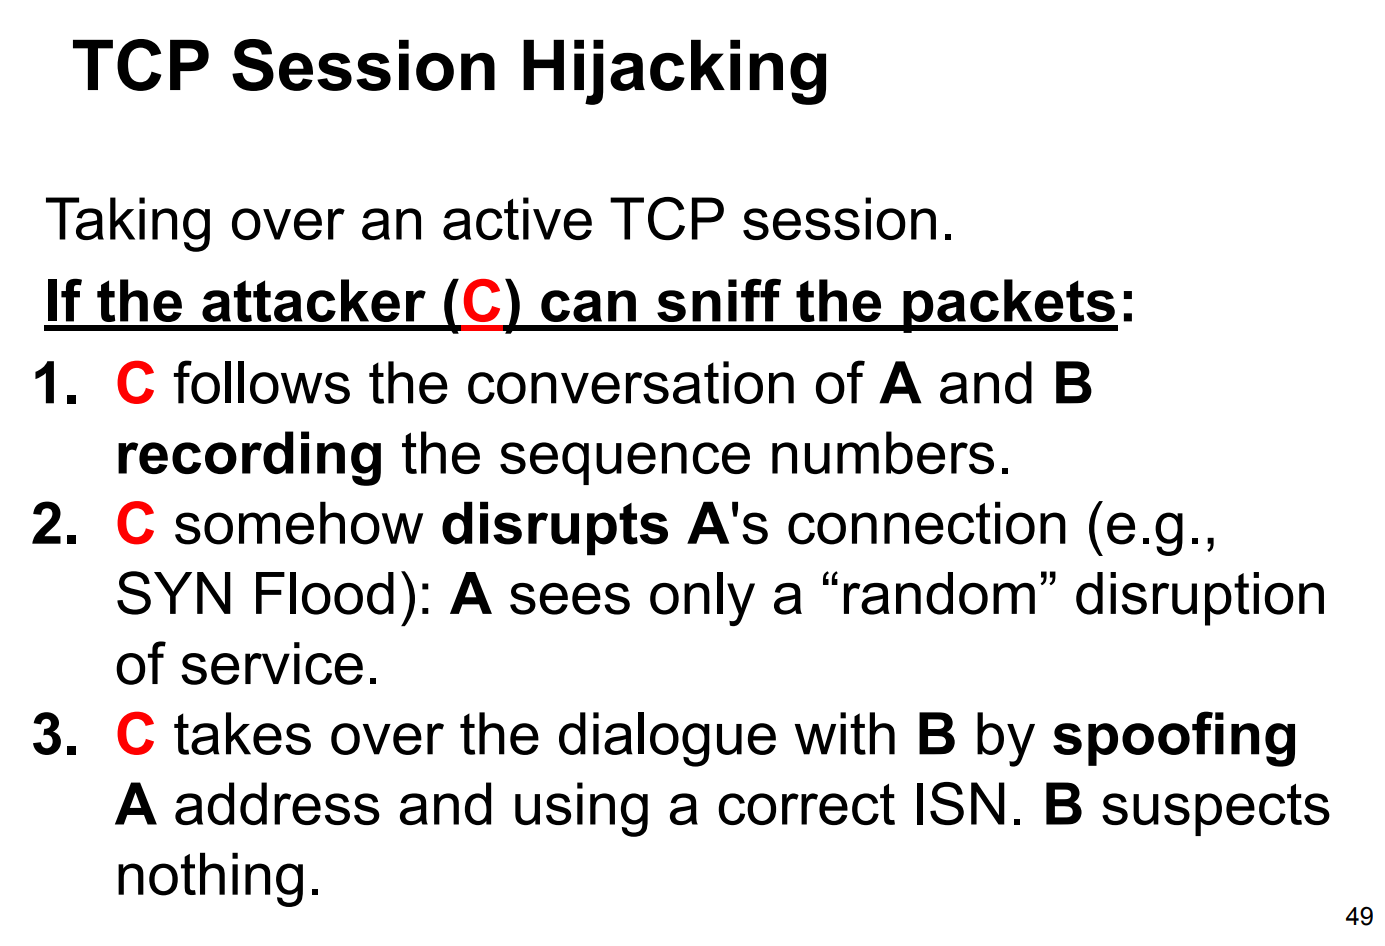
\includegraphics[width=0.8\textwidth]{media/image48.png}
\end{figure}

\begin{figure}[H]
\centering
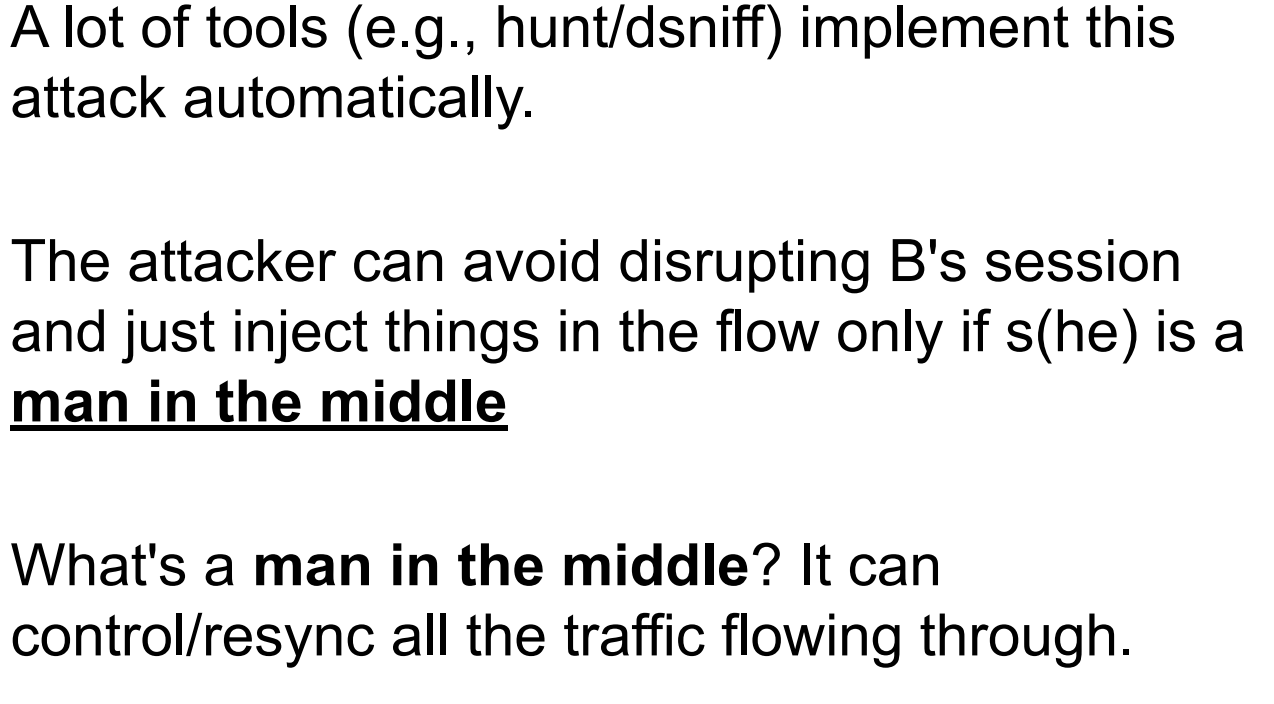
\includegraphics[width=0.8\textwidth]{media/image49.png}
\end{figure}

\subparagraph{Man-in-the-Middle (MITM) attacks}

In a MITM attack, the attacker inserts themselves between two
communicating entities and \textbf{gains full control over the exchanged
traffic}. Instead of interrupting communications, the attacker
transparently intercepts, modifies, redirects, or monitors packets.

MITM attacks are classified into four categories:

\begin{itemize}
\item \textbf{physical MITM;}
\item \textbf{logical MITM;}
\item \textbf{full in-the-loop MITM;}
\item \textbf{out-of-the-loop MITM.}
\end{itemize}

The distinction between full \textbf{in-the-loop} and \textbf{out-of-the-loop}
refers to visibility over communications:

In a \textbf{full in-the-loop} MITM, the attacker can observe both requests
and responses. The attacker has complete control over the communication
channel.

In an \textbf{out-of-the-loop} MITM, the attacker is in a blind position and
can only influence part of the communication, similarly to blind
spoofing attacks.

The distinction between \textbf{physical} and \textbf{logical} MITM instead
concerns the attacker's position.

A \textbf{physical MITM} is a device physically located between two
endpoints, such as a firewall placed between two networks.

A \textbf{logical MITM} is not physically located between the endpoints, but
traffic is logically redirected through the attacker. ARP spoofing is a
perfect example: by pretending to be the gateway, the attacker forces
all traffic to pass through their machine.

\paragraph{DNS Cache Poisoning}

DNS exists because IP addresses and MAC addresses are not user friendly.
Humans cannot realistically remember numerical IP addresses for every
website. DNS therefore maps human-readable domain names to IP addresses.

The DNS infrastructure is hierarchical. A client first checks local
mappings, such as /etc/hosts. If the mapping is absent, the query is
sent to the local DNS server. If the local DNS server does not know the
answer, it recursively or iteratively traverses the DNS hierarchy until
reaching the authoritative DNS server responsible for the target domain.

In recursive resolution, the non-authoritative DNS server resolves the
request on behalf of the client and returns the final mapping.

In iterative resolution, the DNS server instead redirects the client
toward the next authoritative server.

Usually, when a user wants to connect to a website, the local DNS server
checks whether the mapping is already saved in its cache. If the mapping
is not present, the local non-authoritative DNS server contacts the
authoritative DNS server to obtain the correct IP address.

The attack takes advantage of this moment. While the local DNS server is
waiting for the reply from the authoritative DNS server, \hl{the attacker
quickly sends a \textbf{fake DNS response containing a malicious IP
address}}. DNS requests use a query identifier, similar to TCP
sequence numbers, so the attacker must correctly guess this DNS query ID
in order to make the fake response appear legitimate.

If the attacker succeeds, the local DNS server accepts the fake response
and \textbf{stores the malicious mapping inside its cache}. This is why the
attack is called \textbf{DNS cache poisoning}: the cache of the DNS server
becomes poisoned with false information.

From that moment on, every user who asks that DNS server for the address
of example.com will receive the malicious IP address instead of the
legitimate one. As a consequence, users are transparently redirected to
a server controlled by the attacker.

\paragraph{DHCP Spoofing Attack}

The \textbf{DHCP protocol} dynamically assigns network configuration
parameters such as:

\begin{itemize}
\item IP address;
\item subnet mask;
\item gateway;
\item DNS server.
\end{itemize}

DHCP is based on UDP and is not authenticated. The reason is structural:
when a device first joins a network, it does not yet possess the
information necessary to authenticate itself.

This makes DHCP extremely vulnerable. An attacker connected to the same
local network can answer DHCP requests before the legitimate DHCP server
and provide malicious configuration parameters.

For example, the attacker can assign:

\begin{itemize}
\item a malicious gateway;
\item a poisoned DNS server;
\item arbitrary routing information.
\end{itemize}

With a single DHCP spoofing attack, the attacker can effectively prepare
the victim for many additional attacks, including traffic hijacking, DNS
poisoning, and man-in-the-middle attacks.

Again, the attack is feasible only if the attacker belongs to the same
local network.

\paragraph{ICMP Redirect Messages}

Routers use \textbf{ICMP Redirect packets} to inform hosts that a \textbf{better
route exists} for reaching a destination. When a router notices that
traffic could follow a more efficient path, it sends an ICMP Redirect
message suggesting a different gateway.

The problem is that the \hl{authentication mechanism used by ICMP Redirect
is extremely weak.}

The ICMP Redirect packet contains the first eight bytes of the original
payload. The idea is that the host verifies that the redirect
corresponds to one of its own packets.

However, these bytes are not secret. An attacker capable of sniffing
traffic can simply observe the packet, copy the first eight bytes, and
forge a malicious ICMP Redirect message.

As a result, the \textbf{attacker can arbitrarily modify routing tables} and
redirect traffic toward attacker-controlled destinations, enabling:

\begin{itemize}
\item traffic hijacking;
\item sniffing;
\item tampering;
\item denial-of-service attacks.
\end{itemize}

\textbf{Internet-scale routing protocols}, such as BGP, EIGRP, RIP and OSPF,
follow the same general problem seen in other network protocols: they
were mainly designed for efficiency, functionality and connectivity, not
for strong security. For this reason, many of them are weakly
authenticated or not authenticated at all.

\subsection{Conclusions}

\begin{itemize}
\item denial-of-service attacks can never be completely eliminated;
\item most network protocol attacks originate from weak or absent
    authentication;
\item Internet protocols were historically designed for efficiency and
    functionality, not security;
\item many mitigations must be implemented at the operating system or
    software level because changing the protocols themselves would
    require modifying huge portions of the global Internet
    infrastructure while preserving backward compatibility.
\end{itemize}

\section{Secure Network Architectures}

A \textbf{firewall} is a network access control system.

A \textbf{firewall} has \hl{two main functionalities}.

The first one is \textbf{packet filtering}: for each packet, the firewall
applies a set of rules and decides whether that packet can pass or not.

The second functionality is \textbf{network address translation}, or NAT.
This is needed because a firewall often works as an intermediary between
an internal local network and an external network. Therefore, it must
translate internal addresses into external addresses, and vice versa. In
practice, the firewall may rewrite information such as source IP
addresses, ports, and other packet fields.

For a firewall \textbf{to be effective}, it must be \textbf{placed at a single
critical point} between the protected network and the outside network.

If there is another path that bypasses the firewall, then the firewall
becomes \textbf{useless}.

\textbf{However}, firewalls \hl{can only control traffic that passes through
them}. For example, if an attacker has already compromised a
machine inside the local network, that machine may be able to attack or
exfiltrate data from other machines in the same local network without
passing through the firewall.

The same problem appears when there are \textbf{unchecked communication
paths}. Suppose a compromised machine is connected to the LAN but
\end{document}
